\seccion{Variables aleatorias y distribuciones de probabilidad}
\label{Sec:MP:variablealeatoria}

En un experimento  o un dado proceso, los  posibles resultados son t\'ipicamente
n\'umeros  reales, siendo  cada n\'umero  un evento.   Luego los  resultados son
mutuamente  excluyentes. Se  considera  a  esos n\'umeros  como  valores de  una
\emph{variable aleatoria} $X$ a valores reales, que puede ser discreta, continua
o mixta.

Formalmente, la  noci\'on de  variable aleatoria se  apoya sobre la  noci\'on de
funci\'on  medible.  Por  esta  formalizaci\'on, vamos  a  necesitar definir  la
integraci\'on de  manera general,  m\'as all\'a del  enfoque de Riemann  (``a la
Lebesgue''), as\'i  como la noci\'on  de derivada de  una medida con  respecto a
otra para  definir densidades  de probabilidad, en  analog\'ia a la  densidad de
masa en mec\'anica por ejemplo~\cite{Leb04, Leb18, KolFom61, AthLah06, Bog07:v1,
  Coh13}.


% ================================= Medida, integral, densidades

\subseccion{Consideraciones  preliminaries:  Teor\'ias  de  la medida  y  de  la
  integraci\'on.}
\label{Ssec:MP:VAPreliminaria}

La primera noci\'on  que subyace a la definici\'on  formal de variable aleatoria
es la de funci\'on medible:

\begin{definicion}[Funci\'on medible]
\label{Def:MP:FuncionMedible}
%
 Sean  \ $(\Omega,\A)$  \ y  \ $(\Upsilon,\B)$  \ dos  espacios  medibles.  Una
  funci\'on $f: \Omega \mapsto \Upsilon$ se dice {\it $(\A,\B)$-medible} si
  %
  \[
  \forall \,  B \in  \B, \quad  A \equiv f^{-1}(B)  = \left\{  \omega \in  A \tq
    f(\omega) \in B \right\} \: \in \: \A.
  \]
  %
  Dicho de  otra manera, la pre-im\'agen  de un elemento dado  de $\B$ (elemento
  medible) pertenece a $\A$ (elemento medible).  Por abuso de escritura, se dice
  m\'as simplemente que $f: (\Omega,\A) \mapsto (\Upsilon,\B)$ es medible.
\end{definicion}

Adem\'as, a partir de un espacio de medida y una funci\'on $f$ medible, se puede
definir  una  medida  im\'agen   sobre  el  espacio  de  llegada~\cite{AthLah06,
  Bog07:v1, Coh13}:
%
\begin{teorema}[Teorema de la medida im\'agen]
\label{Teo:MP:MedidaImagen}
%
  Sean  \ $(\Omega,\A,\mu)$  \  un espacio  de  medida, \  $(\Upsilon,\B)$ \  un
  espacio  medible  y  $f:  (\Omega,\A)  \mapsto  (\Upsilon,\B)$  una  funci\'on
  medible. Sea $\mu_f$ tal que
  %
  \[
  \forall \,  B \in  \B, \quad  \mu_f(B) = \mu\left( f^{-1}(B) \right).
  \]
  %
  Entonces, $\mu_f$  es una medida  sobre el espacio medible  $(\Upsilon,\B)$, \
  \ie  \  $(\Upsilon,\B,\mu_f)$  \  define  un  espacio  de  medida.   Adem\'as,
  $\mu(\Omega) = \mu_f(\Upsilon)$ (posiblemente  infinitas). Se dice que $\mu_f$
  es la {\it medida im\'agen de $\mu$ por $f$}.
\end{teorema}
%
\begin{proof}
  Por   definici\'on,  claramente   $\mu_f  \ge   0$.    Adem\'as,  obviosamente
  $f^{-1}(\emptyset) =  \emptyset$ \ dando $\mu_f(\emptyset)  = \mu(\emptyset) =
  0$.  Luego,  si para un  conjunto numerable $\{  B_j \}$ de elementos  de $\B$
  disjuntos entre s\'i, las pre-im\'agenes  de los $B_j$ tambi\'en son disjuntos
  entre s\'i  (para $k  \ne j$ no  se puede  tener $\omega \in  f^{-1}(B_j) \cap
  f^{-1}(B_k)$  sino  $\omega$  tendr\'ia  dos im\'agenes  distintas  por  $f$).
  Entonces \ $f^{-1}\left( \bigcup_j B_j \right) = \bigcup_j f^{-1}(B_j)$.  Esto
  implica  que \  $\mu_f\left( \bigcup_j  B_j \right)  =  \mu\left( f^{-1}\left(
      \bigcup_j B_j \right) \right)  = \mu\left( \bigcup_j f^{-1}(B_j) \right) =
  \sum_j  \mu\left(  f^{-1}(B_j)  \right)  =  \sum_j  \mu_f(B_j)$.   Finalmente,
  necesariamente  $f^{-1}(\Upsilon) =  \Omega$ (obviamente  $f(\Omega) \subseteq
  \Upsilon$)  lo  que  cierra  la  prueba~\footnote{De hecho,  se  puede  probar
    sencillamente que la pre-im\'agen de  una uni\'on numerable (disjuntos o no)
    es la uni\'on de las  pre-im\'agenes; lo mismo occure para la intersecci\'on
    y  adem\'as  la  pre-im\'agen  del  complemento  es  el  complemento  de  la
    pre-im\'agen.  Esto se conoce  como {\it leyes de de Morgan}~\cite{AthLah06,
      Coh13,        HogMck13}       (ver       tambi\'en~\cite[Cap.~1]{KolFom57}
    y~\cite[Caps.~5~\&~6]{KolFom61}).\label{Foot:MP:Jacobiana}}
\end{proof}

A  continuaci\'on,  necesitaremos  tratar  de funciones  medibles  teniendo  una
propiedad (P) salvo sobre  un conjunto de medida \ $\mu$ \  igual a cero.  M\'as
generalmente viene ac\'a la noci\'on de propiedad {\it casi siempre}:
%
\begin{definicion}[Propiedad (e igualdad) $\mu$-casi siempre]
\label{Def:MP:CasiSiempre}
%
  Una funcion  medible \  $f$ se  dice tener una  propiedad (P)  dada $\mu$-casi
  siempre, si y solamente si la tiene excepto sobre un conjunto de medida nula,
  %
  \[
  \mu\left( \left\{ \omega  \tq f(\omega) \: \mbox{ no  satisface (P) } \right\}
  \right) = 0.
  \]
  %
  Por ejemplo, dos funciones medibles \ $f_1$ \ y \ $f_2$ \ $(\Omega,\A,\mu) \to
  (\Upsilon,\B)$ \ son iguales $\mu$-casi siempre,
  \[
  f_1 = f_2 \quad (\mu\mbox{-c.s.})
  \]
  %
  si y solamente si son iguales excepto sobre un conjunto de medida nula,
  %
  \[
  \mu\left( \left\{ \omega \tq f_1(\omega) \ne f_2(\omega) \right\} \right) = 0.
  \]
\end{definicion}

\

Un espacio  que juega un rol particular  es $\Rset^d$, al cual  se puede asociar
una  $\sigma$-\'algebra  particular  conocida  como {\it  $\sigma$-\'algebra  de
  Borel}~\cite{AthLah06, Bog07:v1, Bog07:v2, Coh13}:
%
\begin{definicion}[$\Rset^d$ y Borelianos]
\label{Def:MP:Borelianos}
%
  Para  cualquier  $d  \ge  1$  entero,  llamamos  Borelianos  $\B(\Rset^d)$  de
  $\Rset^d$ a  la $\sigma$-\'algebra m\'as peque\~na generada  por los productos
  cartesianos     $\displaystyle    \optimes_{i=1}^d    (-\infty     \;    b_i]$
  \big(similarmente,  por  los  abiertos  de  $\Rset^d$, o  tambi\'en  para  los
  productos  cartesianos de intervalos  $\displaystyle \optimes_{i=1}^d  (a_i \;
  b_i]$\big), \ie uniones numerables, intersecciones numerables, complementos de
  estos intervalos.  $\B(\Rset^d)$  es tambi\'en llamado {\it $\sigma$-\'algebra
    de Borel de $\Rset^d$}.
\end{definicion}

\

Se necesita ahora definir la  noci\'on de integraci\'on de una funci\'on medible
con respecto a una medida:
%
\begin{definicion}[Medida e integraci\'on]
\label{Def:MP:MedidaIntegracion}
%
  Para una medida  cualquiera, sobre un espacio de  medida $(\Omega,\A,\mu)$, se
  define la integraci\'on a partir de
  %
  \[
  \forall \, A \in \A,  \quad \int_A d\mu(\omega) = \int_\Omega \un_A(\omega) \,
  d\mu(\omega) = \mu(A),
  \]
  %
  donde $\un_A$ es la funci\'on indicadora (ver notaciones).
  %
%  \[
%  \un_A(\omega) = \left\{
%  \begin{array}{ccc}
%  1 & \mbox{si} & \omega \in A\\
%  0 & \mbox{si} & \omega \not\in A
%  \end{array} \right.
%  \]
  %
  es  la funci\'on  indicadora del  conjunto $A$.   $d\mu(\omega)$ se  escribe a
  veces tambi\'en $\mu(d\omega)$,  medida de un ``infinit\'esimo''.  Claramente,
  por  propiedades  de una  medida,  para $  A_i,  A_j$  disjuntos $\un_{A_i}  +
  \un_{A_j}  =  \un_{A_i \cup  A_j}$,  dando  $\displaystyle \int_\Omega  \left(
    \un_{A_i} + \un_{A_j} \right) d\mu(\omega)  = \mu(A_i \cup A_j) = \mu(A_i) +
  \mu(A_j)  =   \int_\Omega  \un_{A_i}  d\mu(\omega)   +  \int_\Omega  \un_{A_j}
  d\mu(\omega)$ y entonces, sin perdida  de generalidad para un conjunto $\{ A_j
  \}$ numerable
  %, con los $A_j$ disjuntos,  
  y $\{  a_j \}$ reales no negativos,  la integral de la  funci\'on escalonada \
  $\displaystyle \sum_j a_j \un_{A_j}$ \ es dada por
  %
  \[
  \int_\Omega \left( \sum_j a_j \un_{A_j}(\omega) \right) \, d\mu(\omega) =
  \sum_j a_j \int_\Omega \un_{A_j}(\omega) \, d\mu(\omega).
  \]
  %
  Para  los  $A_i$  disjuntos  es   la  consecuencia  directa  de  la  propiedad
  precedente, y  si $A_i,  A_j$ no son  disjuntos.  De hecho,  sufice considerar
  $A_i\setminus  A_j,  \:  A_j\setminus  A_i,  A_i \cap  A_j$  \  con  \modif{$A
    \setminus B = \{ \omega \tq \omega \in  A \: \y \: \omega \not\in B \}$} \ y
  respectivamente los coefficientes \ $a_i, \: a_j, \: a_i + a_j$ para volver al
  caso de conjuntos disjuntos.
  %
\end{definicion}


Antes de definir la integraci\'on de una funci\'on real, medible, cualquiera, el
\'ultimo paso que falta es el siguiente:
%
\begin{teorema}[Funci\'on medible como l\'imite]
\label{Teo:MP:MedibleLimite}
%
  Sea   \   $g:   (\Omega,\A)   \mapsto  (\Rset,\B(\Rset))$,   no   negativa   y
  medible. Existe  una sucesi\'on  \ $\{  g_n \}_{n \in  \Nset}$ \  creciente de
  funciones escalonadas que converge simplemente (punto a punto) hacia $g$.
\end{teorema}
%
\begin{proof}
  La  sucesi\'on \ $\displaystyle  g_n =  \sum_{k=0}^{n 2^n-1}  \frac{k}{2^n} \,
  \un_{g^{-1}\left( \left[ \frac{k}{2^n} \; \frac{k+1}{2^n} \right) \right)} + n
  \, \un_{g^{-1}\left(  \left[ n \;  +\infty \right) \right)}$ \  es escalonada,
  creciente y converge  hacia $g$ \ (notar que esta  sucesi\'on comparte la idea
  que subyace a la integraci\'on de Riemann).
\end{proof}

De  este resultado, se  puede generalizar  la noci\'on  de integraci\'on  de una
funci\'on real:
%
\begin{definicion}[Integraci\'on de una funci\'on real]
\label{Def:MP:IntegracionReal}
%
  Sea \ $g:  (\Omega,\A) \mapsto (\Rset,\B(\Rset))$, no negativa  y medible, y \
  $\{ g_n \}_{n \in \Nset}$  \ una sucesi\'on creciente de funciones escalonadas
  que converge simplemente hacia $g$. Por definici\'on,
  %
  \[
  \int_{\Omega}  g(\omega) \,  d\mu(\omega)  = \lim_{n  \to \infty}  \int_\Omega
  g_n(\omega) \, d\mu(\omega).
  \]
  %
  Notar  de  que  el  l\'imite  puede  ser infinita.\newline  Sea  ahora  \  $g:
  (\Omega,\A)  \mapsto  (\Rset,\B(\Rset))$ \  medible  cualquiera.  Se  verifica
  sencillamente  que  tambi\'en  $|g|$   (valor  absoluto)  es  medible  y,  por
  definici\'on, $g$ se dice $\mu$-integrable si la integral de $|g|$ es finita,
  %
  \[
  g   \:  \mbox{es}   \:  \mu\mbox{-integrable}   \quad   \Leftrightarrow  \quad
  \int_\Omega |g(\omega)| \, d\mu(\omega) < +\infty.
  \]
  %
  Adem\'as,  se  escribe $g  =  g_+  +  g_-$ con  $g_+  =  \max(g,0)$ y  $g_-  =
  \min(g,0)$. Es sencillo ver de que si \  $g$ \ es medible, \ $g_+$ \ y \ $g_-$
  \ son medibles. Si  \ $g$ \ es $\mu$-integrable, necesariamente \  $g_+$ \ y \
  $g_-$ \ son $\mu$-integrables, y, por definici\'on
  %
  \[
  \int_\Omega   g(\omega)   \,  d\mu(\omega)   =   \int_\Omega  g_+(\omega)   \,
  d\mu(\omega) - \int_\Omega \left( - g_-(\omega) \right) \, d\mu(\omega).
  \]
\end{definicion}

A continuaci\'on, damos  unos teoremas que ser\'an muy  \'utiles m\'as adelante,
sin detallar las pruebas. Por esto, el lector se puede referir a~\cite{LieLos01,
  AthLah06, Bog07:v1, Coh13}.
%
\begin{teorema}[Teorema de convergencia mon\'otona]
\label{Teo:MP:ConvergenciaMonotona}
%
  Sea  \ $\{  f_n \}_{n  \in  \Nset}$ \  una sucesi\'on  creciente de  funciones
  medibles  sobre $(\Omega,\A,\mu)$,  positivas, convergiendo  simplemente hacia
  una funci\'on \ $f$ \ medible. Entonces
  %
  \[
  \lim_{n  \to  +\infty}  \int_\Omega  f_n(\omega)  d\mu(\omega)  =  \int_\Omega
  f(\omega) d\mu(\omega).
  \]
\end{teorema}
%
De   hecho  se   prueba   este  teorema   a   partir  de   la  definici\'on   de
integraci\'on. Este  teorema da una condici\'on  simple permitiendo intercambiar
integraci\'on y l\'imite.

\begin{corolario}
\label{Cor:MP:ConvergenciaDominada}
%
  Sea \ $\{  f_n \}_{n \in \Nset}$ \ una sucesi\'on  de funciones medibles sobre
  $(\Omega,\A,\mu)$,  positivas,   tal  que  la  serie   $\sum_n  f_n$  converge
  simplemente hacia una funci\'on \ $f$, $\mu$-integrable. Entonces
  %
  \[
  \int_\Omega  \sum_{n   \in  \Nset}  f_n(\omega)   d\mu(\omega)  =  \int_\Omega
  f(\omega) d\mu(\omega).
  \]
\end{corolario}
%
Es  una consecuencia  del teorema  de convergencia  mon\'otona,  considerando la
sucesi\'on creciente $\{ \sum_{k=0}^n f_k \}_{n \in \Nset}$.

\begin{teorema}[Teorema de convergencia dominada]
\label{Teo:MP:ConvergenciaDominada}
%
  Sea  \ $\{  f_n \}_{n  \in  \Nset}$ \  una sucesi\'on  creciente de  funciones
  medibles sobre $(\Omega,\A,\mu)$  convergiendo simplemente hacia una funci\'on
  \ $f$, medible.  Suponemos que existe una funci\'on  $\mu$-integrable  \ $g$ \
  que  domina  la  sucesi\'on,  \ie  $\forall  \, \omega  \in  \Omega,  \quad  |
  f_n(\omega) | \le g(\omega)$. Entonces
  %
  \[
  \lim_{n  \to  +\infty}  \int_\Omega  f_n(\omega) \,  d\mu(\omega)  =  \int_\Omega
  f(\omega) \, d\mu(\omega) \le \int_\Omega  g(\omega)  \, d\mu(\omega).
  \]
\end{teorema}
%
Este  teorema  da  una  condici\'on  suficiente  muy \'util  y  muy  usada  para
asegurarse de que se puede intercambiar l\'imite e integraci\'on.

El   \'ultimo  teorema   que  vamos   a  necesitar   permite   intercambiar  dos
integraciones.   Antes,  necesitamos  definir  la noci\'on  de  espacio  medible
producto y medida producto.
%
\begin{definicion}[Espacio medible producto, medida producto]
\label{Def:MP:EspacioMedidaProductos}
%
  Sean dos  espacios de  medida \  $(\Omega_1, \A_1, \mu_1)$  \ y  \ $(\Omega_2,
  \A_2,  \mu_2)$. Llamamos  {\it espacio  medible producto}  $(\Omega ,  \A)$ al
  espacio del  producto cartesiano  $\Omega = \Omega_1  \times \Omega_2$  con la
  $\sigma$-\'algebra  $\A$ generada  por los  productos cartesianos  $A_1 \times
  A_2$ donde $A_i \in \A_i, i  = 1, 2$. Adem\'as, llamamos medida producto $\mu$
  definida sobre $\A$ a la medida  tal que $\forall \: (A_1,A_2) \in \A_1 \times
  \A_2, \quad \mu(A_1 \times A_2) = \mu_1(A_1) \mu_2(A_2)$.
\end{definicion}

\begin{teorema}[Teorema de Fubini]
\label{Teo:MP:Fubini}
%
  Sea  $(\Omega,\A,\mu)$  espacio de  medida  producto  de  \ $(\Omega_1,  \A_1,
  \mu_1)$ \  y \ $(\Omega_2,  \A_2, \mu_2)$ donde  $\mu$ es la  medida producto.
  Sea $f$ una funci\'on integrable sobre $(\Omega,\A,\mu)$ entonces 
  \begin{itemize}
  %
  \item  $\omega_1 \mapsto  f(\omega_1,\omega_2)$  \ es  \ $\mu_1$-integrable  \
    ($\mu_2$-c.s.)  \quad y \quad $\omega_2 \mapsto f(\omega_1,\omega_2)$ \ es \
    $\mu_2$-integrable \ ($\mu_1$-c.s.),
  %
  \item $\displaystyle \omega_1  \mapsto \int_{\Omega_2} f(\omega_1,\omega_2) \,
    d\mu_2(\omega_2)$  \ es  \ $\mu_1$-integrable  \quad y  \quad $\displaystyle
    \omega_2 \mapsto \int_{\Omega_1} f(\omega_1,\omega_2) \, d\mu_1(\omega_1)$ \
    es \ $\mu_2$-integrable.
  \end{itemize}
  %
  Adem\'as,
  %
  \[
  \int_{\Omega_1  \times \Omega_2}  f(\omega) \,  d\mu(\omega)  = \int_{\Omega_1}
  \left(    \int_{\Omega_2}   f(\omega)    \,   d\mu_2(\omega_2)    \right)   \,
  d\mu_1(\omega_1)   =  \int_{\Omega_2}   \left(  \int_{\Omega_1}   f(\omega)  \,
    d\mu_1(\omega_1) \right) \, d\mu_2(\omega_2)
  \]
  %
\end{teorema}
%
\begin{teorema}[Integral a par\'ametro: continuidad y diferenciabilidad]
\label{Teo:MP:IntegralParametro}
%
  Sea $I$ un compacto de $\Rset^d$ y $\{ f(\cdot,t) \}_{t \in I}$ una familia de
  funciones medibles sobre $(\Omega,\A,\mu)$,  tal que \ $t \mapsto f(\omega,t)$
  sea  continua   sobre  $I   \:  (\mu$-c.s.).   Si   existe  una   funci\'on  \
  $\mu$-integrable \ $g$ \ tal que
  %
  \[
  \forall \:  t \in I, \quad  \forall \: \omega \in  \Omega, \quad |f(\omega,t)|
  \le g(\omega),
  \]
  %
  entonces \  $\omega \to  f(\omega,t)$ \ es  $\mu$-integrable y la  funci\'on \
  $\displaystyle  t  \mapsto  \int_\Omega  f(\omega,t)  \,  d\mu(\omega)$  \  es
  continua sobre \ $I$.
  %
  Adem\'as, si \ $f(\omega,\cdot)$ \ es  diferenciable sobre \ $I$ \ y si existe
  una funci\'on $\mu$-integrable \ $h$ \ tal que
  %
  \[
  \forall \: t \in I, \quad  \forall \: \omega \in \Omega, \quad \left\| \nabla_t
    f(\omega,t) \right\| \le h(\omega),
  \]
  %
  donde  $\nabla_t$   indica  el  gradiente,   \ie  el  vector   de  componentes
  $\frac{\partial}{\partial  t_1}  ,  \ldots ,  \frac{\partial}{\partial  t_d}$,
  entonces la  funci\'on \ $\displaystyle  t \mapsto \int_\Omega  f(\omega,t) \,
  d\mu(\omega)$ \ es diferenciable sobre \ $I$, \ y
  %
  \[
  \nabla_t  \int_\Omega  f(\omega,t)  \,  d\mu(\omega)  =  \int_\Omega  \nabla_t
  f(\omega,t) \, d\mu(\omega).
  \]
\end{teorema}
%
B\'asicamente,  este  teorema  es   consecuencia  del  teorema  de  convergencia
dominada.

\

Seguimos esta secci\'on con la noci\'on de derivada de una medida con respecto a
otra, dando una definici\'on muy general de densidad:
%
\begin{definicion}[Densidad de una medida]
\label{Def:MP:DensidadMedida}
%
  Sean  $\mu$  y  $\nu$  dos  medidas  cualesquiera  sobre  un  espacio  medible
  $(\Omega,\A)$.  Si existe una funci\'on  real no negativa \ $p: \Omega \mapsto
  \Rset_+$ \ medible tal que
  %
  \[
  \forall \, A \in \A, \quad \nu(A) = \int_A p(\omega) d\mu(\omega),
  \]
  %
  $p$ \ es llamada densidad de \ $\nu$ \ con respecto a \ $\mu$, denotada
  %
  \[
  p = \frac{d\nu}{d\mu},
  \]
  %
  tambi\'en llamada derivada de Radon-Nikod\'ym.
\end{definicion}

Notar   que dos funciones pueden  cumplir esta definici\'on,  por ejemplo si
son  iguales $\mu$-casi siempre.
%diferentes  en  un conjunto  de  medida  \  $\mu$  \  igual a  cero.  M\'as
%generalmente viene ac\'a la noci\'on de igualdad casi siempre:
%%
%\begin{definicion}[Igualidad $\mu$-casi siempre]
%  Dos funciones  medibles \ $p_1$  \ y \  $p_2$ \ son dichas  iguales $\mu$-casi
%  siempre,
%  %
%  \[
%  p_1 = p_2 \quad (\mu\mbox{-c.s.})
%  \]
%  %
%  si y solamente son iguales excepto sobre un conjunto de medida nula,
%  %
%  \[
%  \mu\left( \left\{ \omega: \: p_1(\omega) \ne p_2(\omega) \right\} \right) = 0.
%  \]
%\end{definicion}
%
%\noindent 
De hecho, si  dos funciones \ $p_1  = p_2 \quad (\mu\mbox{-c.s.})$, y  $C$ es el
conjunto donde no son iguales, siendo de medida nula, 
%notando \  $A \setminus C = \{ \omega: \omega \in
%A \:  \mbox{y} \:  \omega \not\in C\}$,  
de \ $\displaystyle  \int_A p_1(\omega)
d\mu(\omega) =  \int_{A\setminus C} p_1(\omega)  d\mu(\omega) = \int_{A\setminus
  C} p_2(\omega) d\mu(\omega) = \int_A p_2(\omega) d\mu(\omega)$ \ se ve que dos
funciones iguales casi siempre pueden ser  densidad de una medida con respecto a
una otra.

Es sencillo ver que  si $\mu(A) = 0$, necesariamente $\nu(A) =  0$. De eso viene
la noci\'on de absoluta continuidad:
%
\begin{definicion}[Absoluta continuidad]
\label{Def:MP:AbsolutaContinuidad}
%
  Sean  \  $\mu$  \  y  \  $\nu$  \ dos  medidas  sobre  un  espacio  medible  \
  $(\Omega,\A)$.   Se dice que  \ $\nu$  \ es  {\it absolutamente  continua} con
  respecto a \ $\mu$, denotado \[\nu \ll \mu,\] si \ $\forall \: A \in \A, \quad
  \mu(A) = 0 \: \Rightarrow \: \nu(A) = 0$.
\end{definicion}
%
De    hecho,     se    muestra    la    rec\'iproca     de    la    definici\'on
Def.~\ref{Def:MP:DensidadMedida} a trav\'es de lo  que se conoce como teorema de
Radon-Nikod\'ym~\cite{Nik30, AthLah06, Bog07:v1, Coh13}:
%
\begin{teorema}[Radon-Nikod\'ym]
\label{Teo:MP:RadonNikodym}
%
  Sean dos medidas $\mu$ \ y \ $\nu$, entonces
  %
  \[
  \nu \ll \mu \quad \Longleftrightarrow  \quad \nu \: \mbox{ admite una densidad
    con respecto a } \: \mu.
  \]
  %
  Adem\'as, esta densidad $\frac{d\nu}{d\mu}$ es \'unica en el sentido de que si
  dos funciones cumplen la definici\'on, son iguales $\mu$-casi siempre.
\end{teorema}

En todo lo que  sigue, hablaremos de ``la'' densidad de una  medida, salvo si se
necesita expl\'icitamente tener en cuenta esta sutileza.

A  continuaci\'on,  dos  lemas  van  a  ser muy  \'utiles  especialmente  en  el
Cap\'itulo~\ref{Cap:SZ:Informacion},  tratando  con  dos  (o  m\'as)  medidas  y
densidades.
%
\begin{lema}
\label{Lem:RelacionIntegracionDerivadasRadon}
%
  Sean \  $\nu$ \ y \  $\mu$ \ dos medidas  sobre \ $(\Omega,\A)$ \  tales que \
  $\nu \ll \mu$. Entonces, para cualquier funci\'on medible $f$,
  %
  \[
  \int_\Omega   f(\omega)  \,   \frac{d\nu}{d\mu}(\omega)   \,  d\mu(\omega)   =
  \int_\Omega f(\omega) \, d\nu(\omega)
  \]
\end{lema}
%
\begin{proof}
  Tomando \ $f =  \un_A$, de la definici\'on Def.~\ref{Def:MP:DensidadMedida} se
  obtiene
  %
  \[
  \int_\Omega  \un_A(\omega)  \,  \frac{d\nu}{d\mu}(\omega)  \,  d\mu(\omega)  =
  \int_A   \frac{d\nu}{d\mu}(\omega)   \,  d\mu(\omega)   =   \nu(A)  =   \int_A
  d\nu(\omega)
  \]
  %
  Se  cierra  la  prueba   usande  el  teorema~\ref{Teo:MP:MedibleLimite}  y  la
  definici\'on~\ref{Def:MP:IntegracionReal}, tratando $f$  con su parte positiva
  y negativa separadamente.
\end{proof}
%
\begin{lema}
\label{Lem:RelacionesDerivadasRadon}
%
  Sean \ $\nu$, \ $\mu$ \ y \ $\lambda$ \ tres medidas sobre \ $(\Omega,\A)$ \ y
  suponemos \ $\nu \ll \lambda$ \ y \ $\lambda \ll \mu$. Entonces
  %
  \begin{itemize}
  \item $\quad \nu \ll \mu$;
  %
  \item  equivalentemente,  el soporte  (ensemble  de  puntos  que no  anula  la
    funci\'on)  de \  $\displaystyle  \frac{d\nu}{d\mu}$ \  est\'a \  inclu\'ido
    ($\mu$-casi    siempre)    en     el    soporte    de    \    $\displaystyle
    \frac{d\lambda}{d\mu}$;
  %
  \item  $\quad   \displaystyle  \frac{d\nu}{d\lambda}  \frac{d\lambda}{d\mu}  =
    \frac{d\nu}{d\mu} \quad (\mu$-c.s.).
\end{itemize}
\end{lema}
%
\begin{proof}
  El  primer resultado  viene  de  la definici\'on  de  la absoluta  continuidad
  $\mu(A) =  0 \quad  \Rightarrow \quad \lambda(A)  = 0 \quad  \Rightarrow \quad
  \nu(A) =  0$. El  segunndo resultado  se obtiene escribiendo  la medida  en su
  forma integral.   Ad\'emas, por definici\'on de la  densidad, \ $\displaystyle
  \forall  \: A  \in  \A,  \quad \nu(A)  =  \int_A \frac{d\nu}{d\mu}(\omega)  \,
  d\mu(\omega)$.   Luego,   aplicando  el   lema  anterior  a   \  $f   =  \un_A
  \frac{d\nu}{d\mu}$  \ se  obtiene que,  tambi\'en, \  $\displaystyle  \nu(A) =
  \int_A    \frac{d\nu}{d\lambda}(\omega)   \,    d\lambda(\omega)    =   \int_A
  \frac{d\nu}{d\lambda}(\omega)      \,     \frac{d\lambda}{d\mu}(\omega)     \,
  d\mu(\omega)$, lo que cierra la prueba.
\end{proof}

\

Unas medidas que juegan un rol  particular son las medidas de Lebesgue o medidas
discretas.
%
\begin{definicion}[Medida de Lebesgue]
\label{Def:MP:Lebesgue}
%
  La medida de Lebesgue $\mu_L$  sobre $(\Rset^d,\B(\Rset^d))$ se define tal que
  para cualquier producto cartesiano de intervalos,
  %
  \[
  \mu_L\left( \optimes_{i=1}^d (a_i \; b_i) \right) = \prod_{i=1}^d (b_i-a_i).
  \]
  %
\end{definicion}
%
Ac\'a, notamos dos hechos interesantes:
%
\begin{itemize}
%
\item $\mu_L$ es $\sigma$-finita. Viene de $\Rset^d = \cup_{i=1}^d \cup_{j_i \in
    \Zset}   \optimes_{i=1}^d    (   j_i   \;   j_i+1]$    \   conjuntamente   a
  $\mu_L(\optimes_{i=1}^d ( j_i \; j_i+1]) = 1 < +\infty$.
%
\item $\forall \:  A \in \A, \quad  \mu_L(A) = |A|$ volumen de $A$.
% \ donde  $|\cdot|$ denota el  volumen de un conjunto (puede ser infinito).
%
\item Para una funci\'on \ $g$ \ suficientemente ``suave'', la integraci\'on con
  respecto a la medida de Lebesgue coincide naturalmente con la integraci\'on de
  Riemann.
\end{itemize}
%
La medida de  Lebesgue es as\'i natural para la integraci\'on.  Luego, en lo que
sigue, al  mencionar igualdad  $\mu_L$-casi siempre, diremos  simplemente ``casi
siempre'' $(c.s.)$, entendiendo que es con  respecto a la medida de Lebesgue. De
la misma manera, hablando de densidad, sin precisiones, se entender\'a que s con
respecto a $\mu_L$.

Al  ``contrario'' de  la medida  de  Lebesgue, medidas  discretas son  tambi\'en
particulares. La  m\'as ``elemental''  es conocida como  {\it medida  de Dirac},
dando lugar a medidas discretas:
%
\begin{definicion}[Medida de Dirac y medida discreta]
\label{Def:MP:Dirac}
%
  La medida de Dirac al punto \ $x_0$, \ denotada \ $\delta_{x_0}$, \ es tal que
  %
  \[
  \forall   \  B  \in   \B(\Rset^d),  \quad   \delta_{x_0}(B)  =   \un_B(x_0)
  %  =
  %\left\{ \begin{array}{ccc}
  %%
  %1 & \mbox{si} & x_0 \in B\\[2.5mm]
  %%
  %0 & \mbox{si} & x_0 \not\in B
  %%
  %\end{array}\right..
  \]
  %
  Dado un conjunto \ $\X = \{  x_i \}_i$ \ discreto (finito o infinito numerable),
  llamaremos {\it medida discreta} a la medida definida por
  %
  \[
  \mu_\X = \sum_i \delta_{x_i}
  \]
  %
  (en  general,  son definidas  como  combinaciones  lineales positivas,  siendo
  \'este un caso particular).
\end{definicion}
%
Notar que,
% para $f$ medible, tenemos
%
\begin{itemize}
%
\item $\mu_\X$ es  $\sigma$-finita (se muestra con el mismo  enfoque que para la
  medida de Lebesgue).
%
\item $\forall  \: A \in \A,  \quad \mu_\X(A) =  |\X \cap A|$ cardenal de $\X \cap A$.
%\  donde $|\cdot|$
%  denota el cardinal de un conjunto, equivalente discreto del volumen (puede ser
%  infinito tambi\'en).
%
\item Para una funci\'on \ $g$ \ medible,
  \[
  \int_{\Rset^d} g(x) \, d\delta_{x_k}(x) = g(x_k) \qquad \mbox{y} \qquad
  \int_{\Rset^d} g(x) \, d\mu_\X(x) = \sum_{x \in \X} g(x),
  \]
  %
  luego la integraci\'on se  vuelve una suma.  Se prueba saliendo de  \ $g$ \ de
  la   forma  \  $g   =  \un_C$   \  y   del  Teorema~\ref{Teo:MP:MedibleLimite}
  conjuntamente   con  las   definiciones   Def.~\ref{Def:MP:IntegracionReal}  y
  Def.~\ref{Def:MP:Dirac}.
\end{itemize}

\

Con esta  serie de  definiciones, tenemos todo  lo necesario para  introducir la
definici\'on de variables/vectores aleatorios reales y sus caracterizaciones.


% ================================= VA y distribuci\'on de probabilidad

\subseccion{Variables aleatorias y vectores aleatorios. Distribuci\'on de probabilidad.}
\label{Ssec:MP:VAGeneral}

Empezamos con  la noci\'on de variable  aleatoria real, que  corresponde< como el
resultado de un experimento o de un evento dado~\cite{AthLah06, Coh13, Bre88}:
%
\begin{definicion}[Variable aleatoria real]
\label{Def:MP:VariableAleatotiaReal}
%
  Una variable aleatoria real es una funci\'on medible
  %
  \[
  X: (\Omega,\A,P) \mapsto (\Rset,\B(\Rset),P_X)
  \]
  %
  donde la medida  $P_X$ sobre $\B(\Rset)$ es la medida imagen  de $P$.  \ $P_X$
  es frecuentemente llamada {\it distribuci\'on  de probabilidad} o {\it ley} de
  la variable aleatoria $X$. En lo que sigue, escribiremos \modif{para cualquier
    $B \in \B(\Rset)$} los eventos
  %
  \[
  (X \in B) \equiv X^{-1}(B) = \{ \omega \in \Omega \tq X(\omega) \in B \},
  \]
  %
  as\'i que, por definici\'on,
  %
  \[
  P_X(B) = P(X \in B).
  \]
\end{definicion}
%
Para  ilustrar esta definici\'on,  tomando el  ejemplo de  un dado,  $\Omega$ es
discreto y representa las caras,  mientras que los n\'umeros \modif{(se asocia a
  cada  cara  un  n\'umero  real)}   ser\'an  la  imagen  de  $\Omega$  por  $X$
(ej. $X(\omega_j) = j, \quad j = 1, \ldots , 6$).

Notar que, por las propiedades  de una medida sobre una $\sigma$-\'algebra, para
caracterizar completamente la distribuci\'on $P_X$ es suficiente conocerla sobre
los intervalos de la forma $(-\infty \; b]$.  Esto da lugar a la definici\'on de
funci\'on de repartici\'on~\cite{AthLah06, Coh13, Bre88, HogMck13}:
%
\begin{definicion}[Funci\'on de repartici\'on]
\label{Def:MP:FuncionReparticion}
%
La funci\'on de repartici\'on $F_X$ de una variable aleatoria $X$ se define como
  %
  \[
  F_X(x) = P_X((-\infty \; x]) = P(X \le x).
  \]
  %
  A veces, por abuso  de lenguaje, se denomina a $F_X$ {\it  ley} de la variable
  aleatoria.  Se encuentra  tambi\'en en  la literatura  la  terminolog\'ia {\it
    funci\'on densidad cumulativa} (cdf,  por ``cumulative density function'' en
  ingl\'es).
\end{definicion}
%
Naturalmente, de las propiedades de una medida de probabilidad se tiene:
%
\begin{itemize}
\item $0 \le F_X(x) \le 1$;
%
\item $\displaystyle \, \lim_{x \to -\infty} F_X(x) = 0$ y \ $\displaystyle \,
  \lim_{x \to +\infty} F_X(x) = 1$  (viene de $P_X(\emptyset) = 0$ y $P_X(\Rset)
  = 1$);
%
\item $F_X$ es creciente \big(viene de  que \ $x_1 \le x_2 \: \Leftrightarrow \:
  (-\infty \; x_1] \subseteq (-\infty \; x_2]$\big);
%
\item $F_X$ no es necesariamente continua  (lo vamos a ver m\'as adelante); pero
  en cada punto $x$, $F_X$ es continua por la derecha (ver inciso anterior).
\end{itemize}


Cuando se trabaja  con $d \ge 2$ variables aleatorias  es conveniente definir un
{\it vector aleatorio}  de dimensi\'on~$d$, y apelar para  su estudio a nociones
del \'algebra  lineal y  a notaci\'on matricial.   Se tiene el  vector aleatorio
$d$-dimensional \ $X = \begin{bmatrix} X_1 & \cdots & X_d \end{bmatrix}^t$,
%%%%%%%%%%%%
\modif{aca, saque la definicion de la transpuesta porque esta en las notaciones}
%%%%%%%%%%%%
% donde $\cdot^t$ denota la transpuesta,
caracterizado por  $d$-uplas de  variables aleatorias reales.   Como en  el caso
univariado, se define este  vector de la siguiente manera~\cite{AthLah06, Coh13,
  Bre88}:
%
\begin{definicion}[Vector aleatorio real]
\label{Def:MP:VectorAleatorioReal}
%
  Un vector aleatorio real es una funci\'on medible
  %
  \[
  X: (\Omega,\A,P) \mapsto (\Rset^d,\B(\Rset^d),P_X).
  \]
  %
  donde  $\B(\Rset^d)$  son  los  borelianos  de  $\Rset^d$,  $\sigma$-\'algebra
  generada por los productos cartesianos  $(-\infty \; b_1] \times \cdots \times
  (-\infty  \;  b_d]$ y  donde la  medida $P_X$  sobre $\B(\Rset^d)$  es la
  medida  imagen de  $P$  llamada  {\it distribuci\'on  de  probabilidad} de  la
  variable aleatoria (o vector aleatorio) \ $X$. Como en el caso escalar,  \modif{para cualquier
    $B \in \B(\Rset^d)$}
  %
 \[
 (X \in B) \equiv X^{-1}(B) = \{ \omega \in \Omega \tq X(\omega) \in B \} \qquad
 \mbox{y} \qquad P_X(B) = P(X \in B).
 \]
\end{definicion}
%
\noindent Nota: a veces tenemos que considerar el caso de matrices aleatorias, o
funciones  medibles  a  valores  matriciales.    Dado  que  se  puede  poner  en
biyecci\'on  una  matriz  con  un  vector (por  ejemplo  poniendo  cada  columna
``debajo'' de  su columna  antecedente), no desarrollaremos  m\'as este  caso, a
pesar de que a veces sea m\'as  conveniente trabajar con matrices en lugar de su
forma en vector.

\

De las propiedades de una medida sobre una $\sigma$-\'algebra, para caracterizar
completamente la distribuci\'on $P_X$ de nuevo es suficiente conocerla sobre los
elementos de  la forma $\displaystyle  \optimes_{i=1}^d (-\infty \; b_i]$,
\ie  la funci\'on  de repartici\'on  multivariada~\cite{AthLah06,  Coh13, Bre88,
  HogMck13}:
%
\begin{definicion}[Funci\'on de repartici\'on multivariada]
\label{Def:MP:FuncionReparticionMultivariada}
%
  La funci\'on de repartici\'on $F_X$ de  un vector aleatorio $X$ es definida en
  $x = (x_1 , \ldots , x_d)$ por
  %
  \[
  F_X(x) =  P_X\left( \optimes_{i=1}^d (-\infty \; x_i]  \right) = P\left(
    \bigcap_{i=1}^d (X_i \le x_i) \right).
  \]
  %
  Por abuso de notaci\'on, escribiremos en lo que sigue
  \[
  F_X(x) = P(X \le x),
  \]
  %
  dando  por entendido  que  \  $(X \le  x)$  \ es  el  evento \  $\displaystyle
  \bigcap_{i=1}^d (X_i \le x_i)$.
\end{definicion}
%
De nuevo, de las propiedades de una medida de probabilidad surge:
%
\begin{itemize}
\item $0 \le F_X(x) \le 1$;
%
\item  $\displaystyle \,  \lim_{\forall i,  x_i  \to -\infty}  F_X(x) =  0$ y  \
  $\displaystyle \, \lim_{\forall i, x_i \to +\infty} F_X(x) = 1$;
%
\item $F_X$ es creciente con respecto a cada variable $x_i$.
\end{itemize}
%
Para un subconjunto $I_k = (i_1 \, , \,  \ldots \, , \, i_k)$ de $1 \le k \le d$
elementos de  $\{ 1 \; \ldots \;  d \}^k$, $X_{I_k} =  \begin{bmatrix} X_{i_1} &
  \cdots   &   X_{i_k}\end{bmatrix}^t$  es   obviamente   un  vector   aleatorio
$k$-dimensional. Es entonces sencillo ver que
%
\[
F_{X_{I_k}}(x_{I_k}) = \lim_{\forall i \not\in I_k, x_i \to +\infty} F_X(x)
\label{Pagina:MP:MarginalesF}
\]
%
\Big(viene de  que $\bigcap_{j=1}^k (X_{i_j}  \le x_{i_j}) =  \left( \bigcap_{j=1}^k
  (X_{i_j} \le x_{i_j}) \right) \bigcap  \left( \bigcap_{i \not\in I_k} (X_i \in
  \Rset)  \right)$\Big). Esta  funci\'on se llama {\it  funci\'on  de repartici\'on
  marginal} de $F_X$.

Cerramos estas generalidades con el caso de variables independientes:
%
\begin{definicion}[Independencia]
\label{Def:MP:Independencia}
%
  Sean $d$  variables aleatorias  $X_i$ y  $X = \begin{bmatrix}  X_1 &  \cdots &
    X_d  \end{bmatrix}^t$.   Las  $X_i$   son  mutuamente  independientes  si  y
  solamente   si,  para   cualquier  ensemble   de  conjuntos   $B_i  \modif{\in
    \B(\Rset)}$, los eventos $(X_i \in \B_i)$ son mutuamente independientes, \ie
  %
  \[
  P_X\left( \optimes_{i=1}^d B_i \right) = \prod_{i=1}^d P_{X_i}(B_i).
  \]
  %
  Es equivalente a
  %
  \[
  F_X(x) = \prod_{i=1}^d F_{X_i}(x_i).
  \]
  %
  La ley del vector aleatorio se  factoriza en este caso.  Necesariamente, $\X =
  X(\Omega)$ es de  la forma $\displaystyle \X = \optimes_{i=1}^d  \X_i$ \ con \
  $\X_i = X_i(\Omega)$, producto cartesiano.
\end{definicion}
%
\noindent Es importante notar que no es equivalente a tener la independencia por
pares, como lo ilustramos al final de la secci\'on precedente.

\

M\'as  all\'a de  este  enfoque  general, dos  casos  particulares de  variables
aleatorias son  de inter\'es:  las variables discretas  y las continuas.   En el
primer  caso  $X(\Omega)$  es  discreto,  finito  o  no.   En  las  subsecciones
siguientes estudiamos las particularidades de cada caso.

Para fijar notaciones, en todo lo que sigue escribiremos
%
\[
\X = X(\Omega)
\]
%
conjunto de  llegada de $X$, o conjunto  de valores que puede  tomar la variable
aleatoria.   A veces,  por  simplicidad, se  considera  a $\X$  como el  espacio
muestral  y se  olvida  que $X$  sea  una funci\'on  medible  entre espacios  de
probabilidades, \ie se trabaja en $(\Rset^d,\B(\Rset^d),P_X)$ como en el espacio
pre-imagen.



% ================================= Discreta

\subseccion{Variable aleatoria discreta}
\label{Ssec:MP:VADiscreta}

\begin{definicion}[Variable aleatoria discreta]
\label{Def:MP:VariableAleatoriaDiscreta}
%
  Una  variable aleatoria se  dice {\it  discreta} cuando  $\X =  X(\Omega)$ es
  discreto,  finito o  infinito numerable.
\modif{aca saque la notacion del cardenal, porque ya esta en las notaciones}
  % En  lo que sigue, denotaremos  por $|\X|$ al cardinal  de $\X$, posiblemente
  % infinito.
  En otras palabras, los posibles valores de una variable aleatoria discreta $X$
  consisten en un  conjunto contable (finito o infinito  numerable) de n\'umeros
  reales, \  $\X = \{  x_j \}$ \  y se puede  escribir a \  $X$ \ como  una {\it
    variable escalonada} (ver ej.~\cite{AthLah06, HogMck13}),
  %
  \[
  X = \sum_j x_j \un_{A_j} \quad \mbox{con} \quad A_j = X^{-1}(\{ x_j \}).
  \]
\end{definicion}
%
\noindent Notar  que $\Omega$  no es necesariamente  discreto.  Por  ejemplo, si
$\omega$ es la posici\'on de un punto sobre una lin\'ea, y se tiene \ $X(\omega)
=  0$ si  $\omega$ est\'a  a la  izquierda de  un umbral  y $X(\omega)  =  1$ si
$\omega$ est\'a a su derecha, luego $\X = \{ 0 \; 1 \}$ mientras que $\Omega$ no
es discreto.

En el  caso de una variable  aleatoria discreta $X$,  las probabilidades $P_X(\{
x_j \})  = P(X = x_j), \:  x_j \in \X$ caracterizan  completamente esta variable
aleatoria~\cite{AthLah06, HogMck13}:
%
\begin{definicion}[Funci\'on de masa de probabilidad]
\label{Def:MP:MasaProbabilidad}
%
  \modif{Se  define} la  funci\'on  de  masa de  probabilidad  de $X$,  variable
  aleatoria discreta tomando sus valores sobre $\X$ por
  %
  \[
  p_X(x) \equiv P(X = x) = P_X( \{ x\} ) \quad x \in \X.
  \]
  %
  Por   abuso  de   denominaci\'on,  llamaremos   en  este   libro a   $p_X$  {\it
    distribuci\'on de probabilidad}. Adem\'as, usaremos tambi\'en la notaci\'on
  %
  \[
  p_X = \begin{bmatrix} \cdots & p_X(x_i) & \cdots \end{bmatrix}^t
  \]
  %
  que llamaremos {\it vector  de probabilidad}, de tama\~no $|\X|$, posiblemente
  infinito.
\end{definicion}
%
En  la  Fig.~\ref{Fig:MP:ProbaDiscreta}-(a)   se  muestra  una  representaci\'on
gr\'afica de una distribuci\'on de probabilidad discreta.

Notar  que siendo  $P_X$ una  medida de  probabilidad, $p_X  \ge 0$  \  y est\'a
obviamente normalizada en el sentido de que
%
\[
\sum_{x \in \X} p_X(x) = 1.
\]
%
\modif{Dicho de  otra manera, en  el caso finito  $|\X| = \alpha <  +\infty$, el
  vector  de probabilidad  $p_X$  partenece  al simplex  estandar  o simplex  de
  probabilidad $p_X \in \Simp{\alpha-1}$ (ver notaciones).}

\modif{Volviendo a la medida de probabilidad $P_X$ se nota que}
%
\[
\forall \,  B \in  \B(\Rset), \quad  P_X(B) = \sum_{x  \in \X  \cap B}  p_X(x) =
\int_B dP_X(x),
\]
%
lo que da para la funci\'on de repartici\'on
%
\[
F_X(x) = \sum_{x_j \le x} p_X(x_j).
\]
%
De  esta forma,  se justifica  la  denominaci\'on {\it  cumulativa} para  $F_X$.
Tambi\'en, se puede ver de inmediato que $F_X$ es una funci\'on discontinua, con
saltos  finitos (en  $x_j$,  salto  de altura  $p_X(x_j)$).   Esto es  ilustrado
figura~\ref{Fig:MP:ProbaDiscreta}-(b).

\begin{figure}[h!]
\begin{center} \begin{tikzpicture}%[scale=.9]
\shorthandoff{>}
%
\pgfmathsetmacro{\sx}{1.6};% x-scaling 
\pgfmathsetmacro{\r}{.05};% radius arc non continuity F_X
% masa
\begin{scope}
%
\pgfmathsetmacro{\sy}{6};% y-scaling 
%
\draw[>=stealth,->] (-.25,0)--({\sx*sqrt(11)+.75},0) node[right]{\small $x$};
\draw[>=stealth,->] (0,-.25)--(0,{\sy/3+.5}) node[above]{\small $p_X$};
%
\draw (\sx,-.1) node[below,scale=.8]{\small $1$} --(\sx,0);
\draw[dotted] (\sx,0)--(\sx,{\sy/8}) node[scale=.7]{$\bullet$};
\draw (0,{\sy/8})--(-.1,{\sy/8}) node[left,scale=.7]{\small $1/8$};
%
\draw ({\sx*sqrt(3)},-.1) node[below,scale=.8]{\small $\sqrt3$} --({\sx*sqrt(3)},0);
\draw[dotted] ({\sx*sqrt(3)},0)--({\sx*sqrt(3)},{\sy/4}) node[scale=.7]{$\bullet$};
\draw (0,{\sy/4})--(-.1,{\sy/4}) node[left,scale=.7]{\small $1/4$};
%
\draw ({\sx*sqrt(5)},-.1) node[below,scale=.8]{\small $\sqrt5$} --({\sx*sqrt(5)},0);
\draw[dotted] ({\sx*sqrt(5)},0)--({\sx*sqrt(5)},{\sy/6}) node[scale=.7]{$\bullet$};
\draw (0,{\sy/6})--(-.1,{\sy/6}) node[left,scale=.7]{\small $1/6$};
%
\draw ({\sx*sqrt(7)},-.1) node[below,scale=.8]{\small $\sqrt7$} --({\sx*sqrt(7)},0);
\draw[dotted] ({\sx*sqrt(7)},0)--({\sx*sqrt(7)},{\sy/8}) node[scale=.7]{$\bullet$};
%
\draw ({\sx*sqrt(11)},-.1) node[below,scale=.8]{\small $\sqrt{11}$} --({\sx*sqrt(11)},0);
\draw[dotted] ({\sx*sqrt(11)},0)--({\sx*sqrt(11)},{\sy/3}) node[scale=.7]{$\bullet$};
\draw (0,{\sy/3})--(-.1,{\sy/3}) node[left,scale=.7]{\small $1/3$};
%
\draw ({\sx*sqrt(3)},-1) node{\small (a)};
\end{scope}
%
%
% reparticion
\begin{scope}[xshift=8.5cm]
%
\pgfmathsetmacro{\sy}{2.5};% y-scaling 
%
\draw[>=stealth,->] (-.6,0)--({\sx*sqrt(11)+1.5},0) node[right]{\small $x$};
\draw[>=stealth,->] (0,-.25)--(0,{\sy+.5}) node[above]{\small $F_X$};
%
\draw (\sx,0)--(\sx,-.1) node[below,scale=.8]{\small $1$};
\draw ({\sx*sqrt(3)},0)--({\sx*sqrt(3)},-.1) node[below,scale=.8]{\small $\sqrt{3}$};
\draw ({\sx*sqrt(5)},0)--({\sx*sqrt(5)},-.1) node[below,scale=.8]{\small $\sqrt{5}$};
\draw ({\sx*sqrt(7)},0)--({\sx*sqrt(7)},-.1) node[below,scale=.8]{\small $\sqrt{7}$};
\draw ({\sx*sqrt(11)},0)--({\sx*sqrt(11)},-.1) node[below,scale=.8]{\small $\sqrt{11}$};
%
\draw[thick](-.5,0)--(\sx,0);
\draw ({\sx+\r},\r) arc (90:270:\r);
%
\draw[dotted] (\sx,0)--(\sx,{\sy/8});
\draw[thick](\sx,{\sy/8}) node[scale=.7]{$\bullet$}--({\sx*sqrt(3)},{\sy/8});
\draw ({\sx*sqrt(3)+\r},{\r+\sy/8}) arc (90:270:\r);
\draw (0,{\sy/8})--(-.1,{\sy/8}) node[left,scale=.7]{\small $1/8$};
%
\draw[dotted] ({\sx*sqrt(3)},{\sy/8})--({\sx*sqrt(3)},{3*\sy/8});
\draw[thick]({\sx*sqrt(3)},{3*\sy/8}) node[scale=.7]{$\bullet$}--({\sx*sqrt(5)},{3*\sy/8});
\draw ({\sx*sqrt(5)+\r},{\r+3*\sy/8}) arc (90:270:\r);
\draw (0,{3*\sy/8})--(-.1,{3*\sy/8}) node[left,scale=.7]{\small $3/8$};
%
\draw[dotted] ({\sx*sqrt(5)},{3*\sy/8})--({\sx*sqrt(5)},{13*\sy/24});
\draw[thick]({\sx*sqrt(5)},{13*\sy/24}) node[scale=.7]{$\bullet$}--({\sx*sqrt(7)},{13*\sy/24});
\draw ({\sx*sqrt(7)+\r},{\r+13*\sy/24}) arc (90:270:\r);
\draw (0,{13*\sy/24})--(-.1,{13*\sy/24}) node[left,scale=.7]{\small $13/24$};
%
\draw[dotted] ({\sx*sqrt(7)},{13*\sy/24})--({\sx*sqrt(7)},{2*\sy/3});
\draw[thick]({\sx*sqrt(7)},{2*\sy/3}) node[scale=.7]{$\bullet$}--({\sx*sqrt(11)},{2*\sy/3});
\draw ({\sx*sqrt(11)+\r},{\r+2*\sy/3}) arc (90:270:\r);
\draw (0,{2*\sy/3})--(-.1,{2*\sy/3}) node[left,scale=.7]{\small $2/3$};
%
\draw[dotted] ({\sx*sqrt(11)},{2*\sy/3})--({\sx*sqrt(11)},\sy);
\draw[thick]({\sx*sqrt(11)},\sy) node[scale=.7]{$\bullet$}--({\sx*sqrt(11)+1.4},\sy);
\draw (0,\sy)--(-.1,\sy) node[left,scale=.7]{\small $1$};
%
\draw ({\sx*sqrt(5)},-1) node{\small (b)};
\end{scope}
%
\end{tikzpicture} \end{center}
%
\leyenda{Ilustraci\'on de una distribuci\'on  de probabilidad discreta (a), y la
  funci\'on de  repartici\'on asociada (b), con $\X  = \big\{ \, 1  \; \sqrt3 \;
  \sqrt5 \; \sqrt7 \; \sqrt{11} \,  \big\}$ \ y \ $p_X = \protect\begin{bmatrix}
    \frac18 & \frac14 & \frac16 & \frac18 & \frac13 \protect\end{bmatrix}^t$.}
\label{Fig:MP:ProbaDiscreta}
\end{figure}

Un caso especial se tiene cuando un  valor $x_k$ es cierto o seguro, y no ocurre
ninguno de los  otros valores $x_j \  (j \ne k)$. La forma  de la distribuci\'on
es:  \ $p_X(x)  = 1$  \  si \  $x =  x_k$  \ y  $0$ si  no;  el vector  de
probabilidad  se escribir\'a  \ $p_X  = \un_k$ 
%donde $\un_k$  denota el vector 
(ver notaciones; el vector posiblemente  de dimensi\'on infinita).
% de componente  $k$-esima igual a
%1, siendo las otras nulas, lo que  s
See denota tambi\'en  con el {\it s\'imbolo de Kronecker} \  $\delta_{jk} = 1$ \
si \ $j = k$ \ y 0 si  no. En este libro, evitaremos usar este s\'imbolo para no
confundirlo  con la medida  de Dirac.  Sin embargo,  resuelta que  \ $P_X$  \ es
precisamente la medida de Dirac en \ $x_k$ (ver Def.~\ref{Def:MP:Dirac}).


Otra   situaci\'on  particular   es  la   de  {\it   equiprobabilidad}   o  {\it
  distribuci\'on  uniforme} cuando  $|\X|  =  \alpha <  +\infty,  \: \alpha  \in
\Nset^*$.  La  forma de la distribuci\'on  es: \ $p_X(x_j)  = \frac1\alpha \quad
\forall \, j =  1 , \ldots , \alpha$, \ie $p_X  = \begin{bmatrix} \frac1\alpha &
  \cdots &  \frac1\alpha \end{bmatrix}^t$ \ o,  en t\'erminos de  medida, $P_X =
\frac1\alpha  \sum_{j=1}^\alpha \delta_{x_j}$.   La  funci\'on de  repartici\'on
resulta una funci\'on escalonada, con  saltos de altura \ $\frac1\alpha$ en cada
$x_j, \quad j = 1 \, , \, \ldots \, , \, \alpha$.

De manera general, la medida de probabilidad de una variable discreta se escribe
como combinaci\'on convexa de medidas de Dirac,
%
\[
P_X =  \sum_j p_j  \delta_{x_j}, \quad  \mbox{con} \quad p_j =  P(X=x_j) \ge  0, \quad
\sum_j p_j = 1,
\]
%
\noindent \ie como una medida discreta.

\

Para comparar  dos distribuciones discretas  es \'util reordenar cada  vector de
probabilidad permutando  sus elementos hasta listarlos de  forma decreciente. El
vector  reordenado a  partir  de $p$  se  anota $p^\downarrow$,  de  modo que  \
$p^\downarrow_1 \ge  p^\downarrow_2 \ge \ldots \ge  p^\downarrow_\alpha$.  En el
ejemplo del caso con certeza se tiene  \ $p^\downarrow = \begin{bmatrix} 1 & 0 &
  \cdots  &  0 \end{bmatrix}^t$,  mientras  que  la  distribuci\'on uniforme  no
var\'ia.  La comparaci\'on de dos vectores de probabilidad se puede apoyar sobre
la noci\'on de mayorizaci\'on:
%
\begin{definicion}[Mayorizaci\'on]
\label{Def:MP:Mayorizacion}
%
  Un vector  de probabilidad  (distribuci\'on) $p$ mayorizado  por un  vector de
  probabilidad (distribuci\'on) $q$, denotado $p \prec q$, se define como:
  %
  \[
  p   \prec  q   \qquad  \mbox{sii}   \qquad  \sum_{i=1}^k   p_i^\downarrow  \le
  \sum_{i=1}^k q_i^\downarrow \quad \forall \, k = 1 \, , \, \ldots \, \alpha-1,
  \qquad  \mbox{y} \qquad  \sum_{i=1}^\alpha p_i^\downarrow  = \sum_{i=1}^\alpha
  q_i^\downarrow
  \]
  %
  (sienco las \'ultimas sumas iguales a 1).  Si los alfabetos de definici\'on de
  \ $p$  \ y \ $q$  \ son de tama\~nos  diferentes, \ $\alpha$ \  es el tama\~no
  m\'as grande y  la distribuci\'on sobre el alfabeto  m\'as corto es completada
  por  estados  de  probabilidad  0  (ser\'ia  equivalente  a  a\~nadir  estados
  ficticios de probabilidad nula).
\end{definicion}
%
\noindent   Por    ejemplo,   $\begin{bmatrix}   0.40   &   0.30    &   0.20   &
  0.10   \end{bmatrix}^t  \prec   \begin{bmatrix}   0.50  &   0.30   &  0.15   &
  0.05 \end{bmatrix}^t$ \ (ver Fig.~\ref{Fig:MP:mayorizacionplot}-(a)).

Es importante resaltar  que la mayorizaci\'on provee un  {\em orden parcial} (no
total)  entre  distribuciones,  existiendo  pares de  distribuciones  tales  que
ninguna mayoriza a la otra.  Por  ejemplo, $\begin{bmatrix} 0.50 & 0.35 & 0.10 &
  0.05  \end{bmatrix}^t$  \   y  \  $\begin{bmatrix}  0.60  &   0.20  &  0.17  &
  .03   \end{bmatrix}^t$  \   no   se  comparan   por   mayorizaci\'on  \   (ver
Fig.~\ref{Fig:MP:mayorizacionplot}-(b)).

Es  interesante  notar  que  la   siguiente  propiedad  es  v\'alida  para  toda
distribuci\'on $p$ de tama\~no~$\alpha$~\cite[p.~9,
  (6)-(8)]{MarOlk11}:
%
\[
\begin{bmatrix}     \frac1\alpha      &     \frac1\alpha     &      \cdots     &
  \frac1\alpha \end{bmatrix}^t  \ \prec \  p \ \prec  \ \begin{bmatrix} 1 &  0 &
  \cdots & 0 \end{bmatrix}^t.
\]
%
En este  sentido, los  casos particulares de  equiprobabilidad y de  certeza, se
dice  que  son  distribuciones  extremas.  Notamos que  uno  implica  ignorancia
m\'axima  en el  resultado de  la variable  mientras que  el otro  corresponde a
conocimiento completo.

La     relaci\'on      de     mayorizaci\'on     es      ilustrada     en     la
figura~\ref{Fig:MP:mayorizacionplot}, donde  se representan las  sumas parciales
en  funci\'on  de  $k$,  llamadas  {\em curvas  de  Lorentz~\footnote{Se  prueba
    sencillamente      que      estas      curvas     son      crecientes      y
    c\'oncavas.}}~\cite{MarOlk11,  Lor05}.   Gr\'aficamente,   $p  \prec  q$  es
equivalente a tener la curva de Lorentz asociada a $p$ por debajo de la asociada
a $q$.
%
\begin{figure}[h!]
\begin{center} \begin{tikzpicture}%[scale=.9]
\shorthandoff{>}
%
% mayorizacion posible
\begin{scope}
%
\draw[>=stealth,->] (-.25,0)--(4.25,0) node[right]{\small $k$};
\draw[>=stealth,->] (0,-.25)--(0,2.25) node[above]{\small
$\begin{array}{l}\sum_{i=1}^k p^\downarrow_i \\[2mm] \sum_{i=1}^k q^\downarrow_i \end{array}$};
%
\draw[dashed] (.8,3.35)--(1.3,3.35);
\draw (.8,2.55)--(1.3,2.55);
%
\draw[dashed] (0,0)--(1,.8) node[scale=.8]{$\bullet$}
 -- (2,1.4) node[scale=.8]{$\bullet$}
 -- (3,1.8) node[scale=.8]{$\bullet$}
 -- (4,2) node[scale=.8]{$\bullet$};
%
\draw (0,0)--(1,1) node[scale=.8]{$\bullet$}
 -- (2,1.6) node[scale=.8]{$\bullet$}
 -- (3,1.9) node[scale=.8]{$\bullet$}
 -- (4,2) node[scale=.8]{$\bullet$};
%
\foreach \k in {1,...,4} {\draw (\k,0)--(\k,-.1) node[below,scale=.7]{\k};}
\draw (0,2)--(-.1,2) node[left,scale=.7]{1};

\draw (2,-1) node{\small (a)};
\end{scope}
%
% mayorizacion imposible
\begin{scope}[xshift=8.5cm]
%
\draw[>=stealth,->] (-.25,0)--(4.25,0) node[right]{\small $k$};
\draw[>=stealth,->] (0,-.25)--(0,2.25) node[above]{\small
$\begin{array}{l}\sum_{i=1}^k p^\downarrow_i \\[2mm] \sum_{i=1}^k q^\downarrow_i\end{array}$};
%
\draw[dashed] (.8,3.35)--(1.3,3.35);
\draw (.8,2.55)--(1.3,2.55);
%
\draw[dashed] (0,0)--(1,1) node[scale=.8]{$\bullet$}
 -- (2,1.7) node[scale=.8]{$\bullet$}
 -- (3,1.9) node[scale=.8]{$\bullet$}
 -- (4,2) node[scale=.8]{$\bullet$};
%
\draw (0,0)--(1,1.2) node[scale=.8]{$\bullet$}
 -- (2,1.6) node[scale=.8]{$\bullet$}
 -- (3,1.94) node[scale=.8]{$\bullet$}
 -- (4,2) node[scale=.8]{$\bullet$};
%
\foreach \k in {1,...,4} {\draw (\k,0)--(\k,-.1) node[below,scale=.7]{\k};}
\draw (0,2)--(-.1,2) node[left,scale=.7]{1};

\draw (2,-1) node{\small (b)};
\end{scope}
%
\end{tikzpicture} \end{center}
%
\leyenda{Orden parcial por mayorizaci\'on: sumas parciales para $k = 1 \, , \, 2
  \,  , \,  3  \, ,  \,  4$  (a) para  los  vectores de  probabilidades  \ $p  =
  \protect\begin{bmatrix} 0.40  & 0.30 & 0.20 &  0.10 \protect\end{bmatrix}^t$ \
  (l\'inea punteada) y \ $q =  \protect\begin{bmatrix} 0.50 & 0.30 & 0.15 & 0.05
    \protect\end{bmatrix}^t$ \  (l\'inea llena) y \  (b) \ para  los vectores de
  probabilidad  $p  =  \protect\begin{bmatrix}  0.50   &  0.35  &  0.10  &  0.05
    \protect\end{bmatrix}^t$    \    (l\'inea     punteada)    y    \    $q    =
  \protect\begin{bmatrix} 0.60  & 0.20 & 0.17 &  0.03 \protect\end{bmatrix}^t$ \
  (l\'inea llena). En el caso (a), \ $p  \prec q$ \ mientras que en el caso (b),
  \  $p  \not\prec q$  \  y  \  $q \not\prec  p$  \  (no est\'an  ordenadas  por
  mayorizaci\'on).  }
\label{Fig:MP:mayorizacionplot}
\end{figure}


% ================================= Continua

\subseccion{Variable aleatoria continua}
\label{Ssec:MP:VAContinua}

En varios contextos,  una variable aleatoria puede tomar  valores en un conjunto
no numerable, por  ejemplo cualesquiera de los n\'umeros  en cierto intervalo de
la recta  real. Ya  no es  una variable discreta.  En las  variables que  no son
discretas,   el   caso   particular    de   inter\'es   es   el   de   variables
continuas~\cite{AthLah06, HogMck13}:
%
\begin{definicion}[Variable aleatoria continua]
\label{Def:MP:VariableAleatoriaContinua}
%
  Una variable  aleatoria \  $X$ \ se  dice {\it  continua} si su  funci\'on de
  repartici\'on  $F_X$ es  continua sobre  $\Rset$.
\end{definicion}

Cuando  se  puede,  es  conveniente  asociar  una  {\it  funci\'on  densidad  de
  probabilidad} (com\'unmente  anotada por su  sigla en ingl\'es: pdf,  por {\it
  probability density function}).   La definici\'on de tal densidad  se apoya en
la definici\'on~\ref{Def:MP:DensidadMedida} aplicada a la medida de probabilidad
$P_X$:
%
\begin{definicion}[Variable aleatoria que admite una densidad de probabilidad]
\label{Def:MP:VariableAdmitiendoDensidad}
%
  Sea   $X$  una  variable   aleatoria  continua   y  \   $P_X$  su   medida  de
  probabilidad.  Por  definici\'on, se  dice  que  $X$  admite una  densidad  de
  probabilidad con  respecto a una medida  $\mu$ sobre $\Rset$ si  $P_X \ll \mu$
  (teorema  de  Radon-Nikod\'ym~\ref{Teo:MP:RadonNikodym}).\newline En  general,
  nos  enfocamos  en  la  medida  (llamada  de  referencia)  $\mu  =  \mu_L$  de
  Lebesgue. Denotando  $d\mu_L(x) \equiv  dx$, la definici\'on  se reduce  a: Si
  existe una funci\'on no negativa \ $p_X$ \ medible sobre $\Rset$ tal que
  %
  \[
  \forall \, B \in \B(\Rset), \quad P_X(B) = \int_B p_X(x) \, dx,
  \]
  %
  entonces se dice que $X$ {\it admite una densidad} y \ $p_X$ \ es llamada {\it
    densidad de  probabilidad} de $X$ (dando  por entendido ``con  respecto a la
  medida de Lebesgue'').   Notando que $P_X(B) = P_X(B \cap  \X)$, el soporte de
  $p_X$ es  necesariamente $\X = X(\Omega)$  (\ie $p_X(\widebar{\X}) = 0$  \ y \
  $p_X(\X) \ne 0$), y
  %
  \[
  \forall \, B \in \B(\Rset), \quad P_X(B) = \int_{B \cap \X} p_X(x) \, dx.
  \]
  %
  Para la funci\'on de repartici\'on \ $F_X$ tenemos entonces
  %
  \[
  F_X(x) = \int_{-\infty}^x p_X(u) \, du
  \]
  %
  (esta expersi\'on es valids por  cualquier medida $\mu$, densidad con respecto
  a esta  medida de referencia,  e integraci\'on sobre  $(-\infty \; x]$  con el
  ``diferencial'' \ $d\mu(x)$).  Dicho de  otra manera, si $F_X$ es (continua y)
  derivable  sobre $\Rset$,  al menos  por partes,  $X$ admite  una  densidad de
  probabilidad (con respecto a  la medida de Lebesgue) y~\footnote{Recordar que,
    rigurosamente, la igualdad debe ser entendida ``casi siempre''.}
  %
  \[
  p_X(x) = \frac{d F_X(x)}{dx}.
  \]
  %
  Por abuso de terminolog\'ia, en lo que sigue llamaremos a $p_X$ tambi\'en {\it
    distribuci\'on de  probabilidad}, a pesar de  que no tiene  el mismo sentido
  que la masa de probabilidad del caso discreto.
%, y denotaremos $|\X|$ el volumen
%  (o medida de Lebesgue) de $\X$, posiblemente infinito.
\end{definicion}
%
La  escritura  integral de  $F_X$  justifica  de  nuevo la  denominaci\'on  {\it
  cumulativa} para  $F_X$. Adem\'as, se puede  ver por ejemplo que  en este caso
$\displaystyle P(a < X \le b) = \int_a^b p_X(x) \, dx = F_X(b) - F_X(a)$ \ y que
claramente
%
\[
\forall x \in \Rset, \quad P_X(\{x\}) = P(X = x) = 0,
\]
%
esto  es, $\{  x \}$  es de  medida $P_X$  nula.  \modif{Similarmente, cualquier
  conjuntos numerable de $\Rset$ es de medida $P_X$ nula.}

Notar aue  aun cuando $0 \le  F_X \le 1$, \  $p_X$ puede ser mayor  que uno. Por
ejemplo, para  \ $F_X(x)  = 2  \, x \,  \un_{\left[ 0  \; \frac12  \right)}(x) +
\un_{\left[  \frac12  \;  +\infty  \right)}(x)$, que  define  correctamente  una
funci\'on  de   repartici\'on,  \   $p_X(x)  =  2   \un_{\left[  0   \;  \frac12
  \right)}(x)$.  No es  contradictorio en  el  sentido de  que $p_X$  no es  una
probabilidad, sino  que $p_X(x) \, dx$  puede ser visto como  la probabilidad de
hallar a  la variable con  valores en el  ``intervalo infinitesimal entre  $x$ y
$x+dx$''.  Finalmente, la condici\'on de normalizaci\'on se escribe
%
\[
\int_\X p_X(x) \, dx = \int_\Rset p_X(x) \, dx = 1. 
\]

En  la  figura~\ref{Fig:MP:ProbaContinua}-(a)  se muestra  una  representaci\'on
gr\'afica de una  funci\'on densidad de probabilidad para  una variable continua
que  admite  una  densidad,  y en  la  figura~\ref{Fig:MP:ProbaContinua}-(b)  la
funci\'on de repartici\'on correspondiente.
%
\begin{figure}[h!]
\begin{center} \input{TIKZ_MP/DistribucionReparticionContinua} \end{center}
%
\leyenda{Ilustraci\'on de:  (a) una  distribuci\'on de probabilidad  continua, y
  (b) la funci\'on  de repartici\'on asociada, con \  $\X = [0 \; 1)  \cup [2 \;
  3)$ \ y \ $p_X(x) = \frac12 \un_{[0 \; 1)}(x) + \frac{5 (x-2)^{\frac32}}{4} \un_{[2
    \; 3)}(x)$,  \ \ie \  $F_X(x) = \frac{x}{2}  \, \un_{[0 \; 1)}(x)  + \frac12
  \un_{[1 \; 2)}(x)  + \frac{1+(x-2)^{\frac52}}{2} \un_{[2 \; 3)}(x)  + \un_{[3 \;
    +\infty)}(x)$.  }
\label{Fig:MP:ProbaContinua}
\end{figure}

Notar que una variable aleatoria puede  no ser ni continua, ni discreta, como se
ilustra en el ejemplo siguiente:
%
\begin{ejemplo}[Ejemplo de variable mixta]
\label{Ej:MP:Mixta}
%
  Sean  $U$ \  y \  $V$ \  variables continuas,  independientes, de  densidad de
  probabilidad \  $p_U = p_V  = \un_{[0 \; 1)}$  \ ($U$ \  y \ $V$ \  son
  uniformes sobre $[0  \; 1)$) \ y sea \  $X = V \un_{U <  \frac12} + \un_{U \ge
    \frac12}$, \ es decir \ $X(\omega) = V(\omega)$ \ si \ $U(\omega) < \frac12$
  \ y  \ $1$ \  si no.   Entonces de la  f\'ormula de probabilidades  totales, \
  $F_X(x) =  P(X \le x) =  P\left( (X \le x)  \left| \left( U  < \frac12 \right)
    \right.  \right) \,  P\left( U < \frac12  \right) \, + \, P\left(  (X \le x)
    \left|  \left( U  \ge  \frac12 \right)  \right.   \right) \,  P\left( U  \ge
    \frac12 \right) $ \ \ie \ $F_X(x)  = \frac12 P\left( (V \le x) \left| \left(
        U < \frac12  \right) \right.  \right) \, + \, \frac12  P\left( (1 \le x)
    \left|  \left(  U  \ge  \frac12  \right)\right. \right)$.  \  Ahora,  de  la
  independencia de  \ $U$  \ y \  $V$, \  tenemos \ $F_X(x)  = \frac12  F_V(x) +
  \frac12 \un_{[1 \; +\infty)}(x)$ \ es decir
  %
  \[
  F_X(x) = \frac{x}{2} \un_{[0 \; 1)}(x) + \un_{[1 \; +\infty)}(x).
  \]
  %
  Esta     funci\'on    de     repartici\'on    es     representada     en    la
  figura~\ref{Fig:MP:ProbaMixta}: no es discreta ni continua.  Entonces, a pesar
  de que $\X = [0 \; 1]$ \  sea un intervalo real, $X$ no es continua (y tampoco
  puede ser discreta).
  %
  \begin{figure}[h!]
  \begin{center} \begin{tikzpicture}%[scale=.9]
\shorthandoff{>}
%
\pgfmathsetmacro{\sx}{2};% x-scaling
\pgfmathsetmacro{\r}{.05};% radius arc non continuity F_X y/o p_X
%
% % cdf
% \begin{scope}
% %
% \pgfmathsetmacro{\sy}{2};% y-scaling 
% %
% \draw[>=stealth,->] (-.6,0)--({\sx*4+.25},0) node[right]{\small $x$};
% \draw[>=stealth,->] (0,-.25)--(0,{3*\sy/4+.5}) node[above]{\small $p_X$};
% %
% \draw[thick] (-.5,0)--(0,0); \draw (\r,\r) arc (90:270:\r);
% %\draw (0,0)--(0,-.1) node[below,scale=.9]{\small $0$};
% %
% \draw[thick] (0,{\sy/2}) node[scale=.7]{$\bullet$} --(\sx,{\sy/2});
% \draw ({\r+\sx},{\r+\sy/2}) arc (90:270:\r);
% \draw (\sx,0)--(\sx,-.1) node[below,scale=.9]{\small $1$};
% \draw (-.1,{\sy/2}) node[left,scale=.7]{\small $1/2$};
% %
% \draw[dotted] (\sx,{\sy/2})--(\sx,0);
% \draw[thick] (\sx,0) node[scale=.7]{$\bullet$} --({2*\sx},0)--
%  plot[domain=2:3,samples=100] ({\sx*\x},{\sy*3*sqrt(\x-2)/4});
% \draw ({\r+3*\sx},{\r+3*\sy/4}) arc (90:270:\r);
% \draw ({2*\sx},0)--({2*\sx},-.1) node[below,scale=.9]{\small $2$};
% %
% \draw[dotted] ({3*\sx},{3*\sy/4})--({3*\sx},0);
% \draw[thick] ({3*\sx},0) node[scale=.7]{$\bullet$} --({4*\sx},0);
% \draw ({3*\sx},0)--({3*\sx},-.1) node[below,scale=.9]{\small $3$};
% \draw (0,{3*\sy/4})--(-.1,{3*\sy/4}) node[left,scale=.7]{\small $3/4$};
% %
% \draw ({\sx*2.25},-1) node{\small (a)};
% \end{scope}
%
%
% reparticion
\begin{scope}%[xshift=8.5cm]
%
\pgfmathsetmacro{\sy}{2};% y-scaling 
%
\draw[>=stealth,->] (-.6,0)--({\sx*2+.25},0) node[right]{\small $x$};
\draw[>=stealth,->] (0,-.25)--(0,{\sy+.5}) node[above]{\small $F_X$};
%
\draw[thick] (-.5,0)--(0,0)--(\sx,{\sy/2});
 \draw ({\sx+\r},{\sy/2+\r}) arc (90:270:\r);
%
\draw[dotted] (\sx,{\sy/2})--(\sx,\sy);
\draw[thick] (\sx,\sy) node[scale=.7]{$\bullet$} --({2*\sx},\sy);
% (0,{\sy/2}) node[scale=.7]{$\bullet$} --(\sx,\sy)--({2*\sx},\sy);
\draw (\sx,0)--(\sx,-.1) node[below,scale=.8]{\small $1$};
\draw (0,{\sy/2})--(-.1,{\sy/2}) node[left,scale=.7]{\small $1/2$};
\draw (0,\sy)--(-.1,\sy) node[left,scale=.7]{\small $1$};
\end{scope}
%
\end{tikzpicture} \end{center}
  %
  \leyenda{Funci\'on de repartici\'on $F_X(x)  = \frac{x}{2} \un_{[0 \; 1)}(x) +
    \un_{[1 \; +\infty)}(x)$ asociada a \ $X  = V \un_{U < \frac12} + \un_{U \ge
      \frac12}$ \  con \ $U$  \ y \  $V$ \ variables  independientes, continuas,
    uniformes sobre $\X = [0 \; 1)$.   $F_X$ no es tipo escal\'on, as\'i que $X$
    no es  discreta. A pesar  de que $\X =  [0 \; 1]$  \ es un intervalo,  de la
    presencia del salto en $x = 1$ tampoco $X$ es continua.}
  \label{Fig:MP:ProbaMixta}
  \end{figure}
  %
\end{ejemplo}
%\item Sea  $U$ \ variable  continua uniforme sobre $[0  \;  1)$ \ y \  $X =
%  \un_{U \not\in \Qset}$. Claramente  $X$ no es continua, pero $\X =  [0 \;
%  1)   \setminus    \Qset$   \   siendo   no   numerable,    $X$   tampoco   es
%  discreta~\footnote{\SZ{$X = 1$ casi siempre\ldots quizas m\'as adelante}}.
%\end{itemize}


Volvemos a las variables  discretas \ $X$ \ sobre $\X =  \{ x_j \}_j$, de medida
de probabilidad de la forma \  $P_X = \sum_j p_j \delta_{x_j}$.  Considerando la
medida  discreta \  $\mu_\X =  \sum_j  \delta_{x_j}$, es  claro que  \ $P_X  \ll
\mu_\X$.  Entonces,  formalmente, $P_X$  admite una densidad  con respecto  a la
medida discreta $\mu_\X$ y esta densidad, definida sobre $\X$ es $p_X(x) = P(X =
x)$.   A  pesar de  que  sea  una tautolog\'ia,  esto  justifica  que usemos  la
escritura  $p_X$  (min\'uscula)  tanto en  el  caso  discreto  como en  el  caso
continuo,  y que  hablemos (por  abuso de  terminolog\'ia) de  distribuci\'on de
probabilidad en ambos casos.\label{Pagina:MP:DensidadDiscreta}

Recordemos que cualquier medida de  probabilidad (caso continuo o no) se escribe
tambi\'en con una integral \ $\displaystyle  P_X(B) = \int_B dP_X(x)$ \ y que en
el caso  discreto cierto \ $X  = x_k$, \ la  medida de probabilidad  $P_X$ es la
medida  de Dirac. A  veces, por  abuso de  escritura \  $dP_X(x)$ es  denotado \
$\delta_{x_k}(x) \,  dx$ \ o \ $\delta(x-x_k)  \, dx$ \ donde  ahora $\delta$ es
llamada {\it distribuci\'on (delta) de Dirac}.  Se puede ver este Dirac como una
densidad de probabilidad  $p_X(x)$ con respecto a la medida  de Lebesgue pero no
es una funci\'on ``ordinaria'' dado que $P_X$ no es diferenciable con respecto a
la  medida  de  Lebesgue.  Se  la  llama  {\it  funci\'on generalizada}  o  {\it
  distribuci\'on de Schwartz}~\footnote{La  teor\'ia de distribuciones vali\'o a
  Laurent Schwarz la  medalla Fields en 1950.  Entre  otros trabajos, se prob\'o
  que el Dirac, visto como  distribuci\'on de Schwartz o funci\'on generalizada,
  tiene   una  ``representaci\'on  integral''   \  $\displaystyle   \delta(x)  =
  \frac{1}{2\pi}  \int_{-\infty}^{\infty}   e^{\imath  t   x}  dt$  \   o  m\'as
  rigurosamente transformada  de Fourier de $x  \mapsto 1$ en el  sentido de las
  funciones  generalizadas   o  distribuciones.   Esto   muestra  claramente  su
  car\'acter no ordinario  (la integral siendo divergente en  el sentido usual).
  Esto va m\'as all\'a de la meta  del cap\'itulo y el lector se podr\'a referir
  a~\cite{Sch66, GelShi64,  GelShi68} por  ejemplo.}.  En particular,  $F_X(x) =
\un_{\Rset_+}(x-x_k)$ \modif{($\un_{\Rset_+}$ es conocido tambi\'en como {\it funci\'on
  de  Heaviside}~\footnote{\modif{Viene del  nombre del  f\'isico  ingles Oliver
    Heaviside quien estudio las ecuaciones electromagneticas de Maxwell.}})} y en
el sentido de las  distribuciones, $\frac{d F_X}{dx} = \delta_{x_k}$.  Adem\'as,
se usan  en general las propiedades,  para cualquier function  \ $f$ \ y  real \
$x_0$,
%
\[
f(x) \delta(x-x_0) = f(x_0) \delta(x-x_0) \qquad \mbox{y} \qquad \int_\Rset f(x)
\delta(x-x_0) \, dx = f(x_0),
\]
%
pero hay que entender la integraci\'on a trav\'es de la medida Dirac (insistimos
en   el   hecho   de  que   esta   notaci\'on   es   un  abuso   de   escritura,
ej.~\cite{GelShi64}).  Usando las distribuciones  de Dirac, se puede unificar el
tratamiento  de  las  variables   aleatorias  discretas  con  las  continuas  en
t\'erminos de densidad  (con respecto a la medida de  Lebesgue): si una variable
aleatoria discreta toma los valores \ $x_j$  \ con probabilidades \ $p_j = P(X =
x_j)$ \  respectivamente, entonces formalmente  se puede describir  mediante una
variable aleatoria continua \ $X$ \ con ``funci\'on densidad de probabilidad'' \
$p_X(x)  =  \sum_j  p_j  \,  \delta(x-x_j)$.   Insistimos en  el  hecho  de  que
rigurosamente  debemos  trabajar  con  medidas,  como lo  hemos  formalizado  al
principio de este cap\'itulo.

Terminamos mencionando el  resultado siguiente, probado en~\cite[Ec.~(2.5)~p.~47
\& teorema~4.1.1]{AthLah} por  ejemplo~\footnote{B\'asicamente, se muestra que \
  $\displaystyle  \widetilde{X}  =  \{ x  \in  \X  \tq  \quad  p(x) =  F_X(x)  -
  \liminf_{u  \to  x}  F(u)  >  0  \}$ \  es  numerable.   A  continuaci\'on,  \
  $\displaystyle F(x) - \sum_{\widetilde{x} \in \widetilde{\X}} p(\widetilde{x})
  \un_{(-\infty  \;  \widetilde{x}]}(x)$  \   es  continua,  y  se  recupera  la
  descomposici\'on    con   $\displaystyle    a   =    \sum_{\widetilde{x}   \in
    \widetilde{\X}} p(\widetilde{x})$.}:
%
\begin{teorema}[Descomposici\'on de una medida de probabilidad]
\label{Teo:MP:DescompositionMixta}
%
  Cualquier  funci\'on  de  repartici\'on   \  $F_X(x)$  \  se  descompone  como
  combinaci\'on convexa  de una funci\'on de repartici\'on  \ $F_{\mathrm{d}}$ \
  discreta y una funci\'on de repartici\'on \ $F_{\mathrm{c}}$ \ continua:
  %
  \[
  \exists  \:  a \in  [0  \; 1]  \quad  \mbox{tal  que}  \quad F_X(x)  =  a
  F_{\mathrm{d}}(x) + (1-a) F_{\mathrm{c}}(x)
  \]
  %
  En  t\'erminos de  medida, o  como  corolario de~\cite[teorema~4.1.1]{AthLah},
  cualquier  medida de probabilidad  $P_X$ se  descompone como  la combinaci\'on
  convexa   de   una   medida   discreta   $P_{\mathrm{d}}$   y   una   continua
  $P_{\mathrm{c}}$,
  %
  \[
  \exists \:  a \in [0  \;  1], \: \widetilde{\X} \:  \mbox{discreto} \quad
  \mbox{tal  que} \quad  P_X  =  a P_{\mathrm{d}}  +  (1-a) P_{\mathrm{c}}  \qquad
  \mbox{con} \qquad P_{\mathrm{d}} \ll \mu_{\widetilde{\X}} \quad \mbox{y} \quad
  P_{\mathrm{c}} \ll \mu_L
  \]
  %
  Entonces, \ $P_X \ll \mu_{\widetilde{\X}}  + \mu_L$, \ \ie admite una densidad
  con respecto a la medida $\sigma$-finita $\mu_{\widetilde{\X}} + \mu_L$.
\end{teorema}
%
Dicho  de  otra manera,  cualquier  variable aleatoria  es  mixta,  como en  el
ejemplo~\ref{Ej:MP:Mixta}.
% pagina~\pageref{Ej:MP:Mixta}. 
Del teorema, es discreta cuando $a = 1$, y continua cuando $a = 0$.


% ================================= Vector discreto

\subseccion{Vector aleatorio discreto}
\label{Ssec:MP:VecDiscreto}

Un ejemplo de vector aleatorio discreto  puede ser dado por un conjunto de dados
(que podr\'ian ser dependientes si est\'an ligados por un hilo por ejemplo).

\begin{definicion}[Vector aleatorio discreto]
\label{Def:MP:VectorAleatorioDiscreto}
%
  Un vector  aleatorio $d$-dimensional se escribe  \ $X =  \begin{bmatrix} X_1 &
    \cdots &  X_d \end{bmatrix}^t$ \ y  \ $\displaystyle \X  = X(\Omega) \subset
  \optimes_{i=1}^d \X_i$ \ donde \ $\X_i =  X_i(\Omega)$. Se dice que \ $X$ \ es
  {\it discreto} cuando $\X \subseteq \Nset^d$, \ es discreto, finito o infinito
  numerable.
  %  En lo  que sigue,  denotaremos tambi\'en  por $|\X|$  el cardinal  de $\X$,
  % posiblemente infinito.
\end{definicion}

Obviamente, la  medida de probabilidad  en los $\displaystyle  x = (x_1 \,  , \,
\ldots \, , \, x_d)  \in \optimes_{i=1}^d \X_i$ \ caracteriza completamente este
vector aleatorio:
%
\begin{definicion}[Funci\'on de masa de probabilidad conjunta]
\label{Def:MP:FuncionMasaConjunta}
%
  Por  definici\'on,  la  funci\'on  de  masa de  probabilidad  de  $X$,  vector
  aleatorio discreto que toma sus  valores sobre $\X \subset \optimes_i \X_i$, \
  est\'a dada por
  %
  \[
  p_X(x) \equiv  P(X =  x) =  P\left( \bigcap_{i=1}^d \left(  X_i =  x_i \right)
  \right) \quad \forall \, x_i \in \X_i, \: 1 \le i \le d.
  \]
  %
  Se la llama  tambi\'en {\it funci\'on de masa de  probabilidad conjunta de los
    $X_i$} o, por  abuso de denominaci\'on,  llamaremos  a $p_X$ {\it
    distribuci\'on  de probabilidad  (conjunta)}.   Notar  que  $\X$ no  es
  necesariamente igual al  producto cartesiano de los $\X_i$.\newline
  %,  de hecho una probabilidad  conjunta para  este producto  puede ser  nula.\newline 
  En el  caso multivariado, la notaci\'on  vectorial es m\'as  delicada de usar:
  $p_X$ ser\'ia un ``tensor'' \modif{(o tabla)} $d$-dimensional (una matriz para
  $d  = 2$,  \modif{una ``tabla''  3  dimensonal para  $d=3$,\ldots}).  Pero  es
  posible  usar una  notaci\'on vectorial,  recordando que  $\Nset^d$  puede ser
  puesto  en  biyecci\'on  con  $\Nset$,  y dada  una  biyecci\'on  usarla  para
  etiquetar los  componentes de $p_X$  puestos en vector.   En el caso  finito \
  $\X_i = \{ x_{j_i} \}_{j=1}^{\alpha_i}$ \ con \ $\alpha_i = |\X_i| < +\infty$,
  \ se puede organizar los componentes tales que $p_X(x_{j_1}\, , \, \ldots \, ,
  \,   x_{j_d})$   sea   la   $j$-esima   componente  del   vector   $p_X$   con
  \modif{$\displaystyle  j =  1  +  \sum_{i=1}^d (j_i  -  1) \,  \prod_{k=i+1}^d
    \alpha_k$}.
%   \  con  \   $\displaystyle  \prod_{k=0}^1  \equiv  1$   \  por
%  convenci\'on.
\end{definicion}
%
\noindent  De  nuevo,  \modif{se  puede  interpretar $p_X$}  como  densidad  con
respecto a la medida discreta $\mu_\X$, Def.~\ref{Def:MP:Dirac}.

\modif{Similarmente al caso  escalar $d = 1$}, la  funci\'on de repartici\'on de
un   vector  aleatorio   discreto  $d$-dimensional   \modif{es   tipo  escal\'on
  $d$-dimensional,  \ie compuesto de  partes de  hiperplanos $d$-dimensionales,
$F_X$   constante  sobre   $[x_{(j-1)_1}  \;   x_{j_1})  \times   \cdots  \times
[x_{(j-1)_d}   \;  x_{j_d})$.}    Adem\'as,  las   componentes   son  mutuamente
independientes si y solamente si la funci\'on de r\'epartici\'on se factoriza, o
equivalentemente la funci\'on de masa se factoriza, \ie
%
\[
X_i  \:  \mbox{mutuamente  independientes}  \quad \Leftrightarrow  \quad  p_X  =
\modif{\prod_{i=1}^d p_{X_i}}.
\]
%
En  notaci\'on  tensorial,  $p_X  =  p_{X_1} \otimes  \cdots  \otimes  p_{X_d}$,
\modif{producto de Kronecker (ver notaciones)}.
% donde $\otimes$  denota el producto tensorial o externo  entre los vectores de
%    probabilidades~\footnote{``Tensor''    $d$-dimensional    de    componentes
%   $(j_1,\ldots,j_d)$  el producto $\prod_i  p_{X_i} (x_{j_i})$.}.   Cuando los
%  $\alpha_i$  son  finito y  la  notaci\'on  vectorial  de la  definici\'on  es
% adoptada, esta expresi\'on queda valide donde $\otimes$ representa el producto
%  de   Kronecker~\footnote{Para  \  $p   =  \begin{bmatrix}  p_1  &   \cdots  &
%     p_n  \end{bmatrix}^t$  \  y  \   $q  =  \begin{bmatrix}  q_1  &  \cdots  &
%     q_m  \end{bmatrix}^t$, \ el  producto de  Kronecker est\'a  dado por  \ $p
%   \otimes q$ \  vector de tama\~no $n m$  de componente \ $\left[ (j-1)  m + k
%   \right]$-esima igual al producto  \ $p_j q_k$ \ para \ $1 \le  j \le n, \: 1
%   \le  k  \le  m$.   Notar  que   este  producto  es  asociativo  pero  no  es
%   conmutativo.\label{Foot:MP:Kronecker}}.

Al  final, de la  f\'ormula de  calculo de  funci\'on de  repartici\'on marginal
vista en la secci\'on~\ref{Ssec:MP:VAGeneral},
% la pagina~\pageref{Pagina:MP:MarginalesF}, 
para un subconjunto $I_k = (i_1,\ldots,i_k)$ de $1 \le k \le d$ elementos de $\{
1  \;  \ldots  \;  d  \}^k$,  $X_{I_k} =  \begin{bmatrix}  X_{i_1}  &  \cdots  &
  X_{i_k}\end{bmatrix}^t$    \modif{tiene   como}   probabilidad    marginal   o
distribuci\'on marginal
% de $X_{I_k}$ es dada por
%
\[
p_{X_{I_k}}(x_{I_k}) = \sum_{\forall i \not\in I_k, x_i \in \X_i} p_X(x).
\]



% ================================= Vector continuo

\subseccion{Vector aleatorio continuo}
\label{Ssec:MP:VecContinuo}

Como  para el  caso de  una variable,  se puede  considerar cualquier  medida de
referencia  $\mu$  sobre  $\Rset^d$   para  definir  una  noci\'on  de  densidad
($d$-variada), pero en general nos enfocamos en la medida de Lebesgue.

\begin{definicion}[Vector   aleatorio  continuo   y  densidad   de  probabilidad
  multivariada]
\label{Def:MP:VectorAleatorioContinuo}
%
  Un vector aleatorio \ $X = \begin{bmatrix} X_1 & \cdots & X_d \end{bmatrix}^t$
  \ se  dice {\it continuo} si  su funci\'on de repartici\'on  $F_X$ es continuo
  sobre      $\Rset^d$.      Como      en     el      caso      escalar,     por
  definici\'on~\ref{Def:MP:DensidadMedida}  (y la rec\'iproca  evocaca despu\'es
  de la definici\'on), se dice que $X$ admite una densidad de probabilidad $p_X$
  con respecto a  una medida $\mu$ sobre $\Rset^d$ si $P_X  \ll \mu$.  De nuevo,
  nos enfocamos en la medida (llamada  de referencia) $\mu = \mu_L$ de Lebesgue:
  si existe una funci\'on no negativa y medible \ $p_X: \Rset^d \mapsto \Rset$ \
  tal que
  %
  \[
  \forall \,  B \in \B(\Rset^d),  \quad P_X(B) =  \int_B p_X(x) \, dx  = \int_{B
    \cap \X} p_X(x) \, dx
  \]
  %
  con $\X  = X(\Omega)$ soporte  de \ $p_X$  \ y \  $d\mu_L(x) \equiv dx  = dx_1
  \cdots dx_d$,  entonces se dice que $X$  {\it admite una densidad}  y $p_X$ es
  llamada {\it densidad de probabilidad}  de \ $X$ (entendiendo ``con respecto a
  la medida de Lebesgue''), o  tambi\'en {\it densidad de probabilidad conjunta}
  de los \ $X_i$. En particular,
  %
  \[
  F_X(x) =  \int_{\optimes_{i=1}^d (-\infty \; x_i]} p_X(u) \, du
  \]
  %
  o, equivalentemente,  para $F_X$ (continua  y) derivable sobre  $\Rset^d$ (con
  respecto a la medida de Lebesgue), por lo menos por partes,
  %
  \[
  p_X(x) = \frac{\partial^d F_X(x)}{\partial x_1 \cdots \partial x_d}.
  \]
  %
  Usaremos   la   terminolog\'ia  (por   abuso)   de   {\it  distribuci\'on   de
    probabilidad}.
  % y denotaremos  todav\'ia \ $|\X|$ \ el  volumen (o medida de  Lebesgue) de \
  % $\X$, posiblemente infinito.
\end{definicion}

Como en el caso  escalar, $p_X \ge 0$ \ (no es necesario que  sea menor que 1) y
satisface la condici\'on de normalizaci\'on
%
\[
\int_\X p_X(x) \, dx = \int_{\Rset^d} p_X(x) \ dx  = 1.
\]

El                                      teorema~\ref{Teo:MP:DescompositionMixta}
%,pagina~\pageref{Teo:MP:DescompositionMixta}    
se cumple tambi\'en en el caso $d$-dimensional: cualquier medida de probabilidad
\  $P_X$  (resp.  funci\'on  de  repartici\'on \  $F_X$)  \  se descompone  como
combinaci\'on  convexa  de  una  medida  de probabilidad  (resp.   funci\'on  de
repartici\'on)  discreta  y una  continua.   En  otros  t\'erminos existe  un  \
$\widetilde{X}$ \  discreto tal que \  $P_X \ll \mu_{\widetilde{\X}}  + \mu_L \:
(\sigma$-finita).

Mencionamos que las $d$ variables  aleatorias $X_1, \ldots, X_d$, componentes de
un vector  aleatorio $X$, son independientes  si y solamente si  la funci\'on de
repartici\'on se factoriza, lo que da, derivando esta,
%
\[
X_i \:  \mbox{ mutuamente independientes} \quad \Leftrightarrow  \quad p_X(x) =
\modif{\prod_{i=1}^d p_{X_i}(x_i)}.
\]


Seguimos esta secci\'on mencionando que, de la f\'ormula de c\'alculo de funci\'on
de  repartici\'on marginal vista en la secci\'on~\ref{Ssec:MP:VAGeneral},
%  pagina~\pageref{Pagina:MP:MarginalesF}, 
para un subconjunto $I_k = (i_1 \, , \,  \ldots \, , \, i_k)$ de $1 \le k \le d$
elementos de  $\{ 1 \; \ldots \;  d \}^k$, $X_{I_k} =  \begin{bmatrix} X_{i_1} &
  \cdots & X_{i_k}\end{bmatrix}^t$ \modif{tiene la} {\it densidad de probabilidad marginal}
% de $X_{I_k}$ es dada por
%
\[
p_{X_{I_k}}(x_{I_k})  = \int_{\times_{i  \not\in  I_k} \X_i}  p_X(x) \,  \prod_{i
    \not\in I_k}  dx_i =  \int_{\Rset^{d-k}} p_X(x) \,  \prod_{i \not\in
      I_k} dx_i.
\]
%
En particular, la funci\'on densidad  de probabilidad marginal que caracteriza a
la variable aleatoria  $X_i$ es la ley que se obtiene  integrando la densidad de
probabilidad conjunta sobre todas las variables excepto la $i$-\'esima.

\

Como  en  el caso  discreto,  se puede  querer  comparar  dos distribuciones  de
probabilidad, y  por eso  reordenar o rearreglar  una densidad  de probabilidad.
Como en el caso discreto, denotamos $p_X^\downarrow$ a la densidad con rearreglo
sim\'etrico.   Primero,  se necesita  definir  el  rearreglo  sim\'etrico de  un
ensemble y luego de una densidad de probabilidad:
%
\begin{definicion}[Rearreglo sim\'etrico de un conjunto]
\label{Def:MP:RearregloConjunto}
%
  Sea $\P \subset \Rset^d$ abierto de  volumen finito, $|\P| < +\infty$.  El {\it
    rearreglo sim\'etrico} $\P^\downarrow$  de $\P$ es la bola  centrada en 0 de
 igual volumen que $\P$, \ie
  %
  \[
  \P^\downarrow  =   \left\{  x   \in  \Rset^d  \tq   \frac{2  \pi^{\frac{d}{2}}
      \|x\|^d}{\Gamma\left(\frac{d}{2}\right)} \modif{<} |\P| \right\} = \Bset_d\left(
    0  \,  , \,  \frac1{\sqrt{\pi}}  \left(  \frac{|\P| \Gamma\left(  \frac{d}{2}
        \right)}{2} \right)^{\frac1d} \right),
  \]
  %
  Esto se ilustra en la figura~\ref{Fig:MP:ensemblerearreglado}-a.
\end{definicion}


\begin{definicion}[Rearreglo sim\'etrico de una densidad de probabilidad]
\label{Def:MP:RearregloDensidad}
%
  Sea $p_X$ una densidad  de probabilidad y sean $\P_t = \{ y  \tq p_X(y) > t \}
  \modif{\subset \Rset^d}$ para cualquier $t > 0$, sus conjuntos de niveles.  La
  densidad de  probabilidad con rearreglo sim\'etrico  $p^\downarrow_X$ de $p_X$
  se  define   como~\footnote{Se  prueba   que  esta  funci\'on,   positiva  por
    definici\'on, suma a 1.   Adem\'as, por construcci\'on, depende \'unicamente
    de $\|x\|$ y decrece con $\|x\|$.}
  %
  \[
  p^\downarrow_X(x)  =  \int_0^{+\infty}  \un_{\P_u^\downarrow}(x) \,  du.
  \]
  %
  %  (recuerdense  de que  $\un_A$  es  el indicator  del  conjunto  $A$) ,  \ie
  % $\un_A(x) = 1$ si $x \in A$ y cero sino.
\end{definicion}
%
De  \ $\forall  \, t  < \tau  \: \Leftrightarrow  \: \P_\tau  \subseteq  \P_t \:
\Leftrightarrow  \: \P_\tau^\downarrow  \subseteq \P_t^\downarrow$,  es sencillo
ver que si $x \in  \P_\tau^\downarrow$, entonces $x \in \P_t^\downarrow$, lo que
conduce  a  $p_X^\downarrow(x)  >  \tau$,  y vice-versa.   M\'as  all\'a,  sobre
$\P_{\tau+d\tau} \setminus  \P_\tau$ la  funci\'on $p_X$ ``vale''  $\tau$ \  y \
sobre  $\P_{\tau+d\tau}^\downarrow  \setminus  \P_\tau^\downarrow$ la  funci\'on
$p_X^\downarrow$  ``vale''   tambi\'en  $\tau$,  lo  que   da  \  $\displaystyle
\int_{\P_\tau^\downarrow} p_X^\downarrow(x) \, dx = \int_{\P_\tau} p_X(x) \, dx$
\  (ver~\cite{LieLos01,   WanMad04}  para   une  prueba  m\'as   rigurosa).   La
representaci\'on de  la definici\'on es conocida como  representaci\'on tarta en
capas  (``layer cake  representation''  en  ingles).  Esto  es  ilustrado en  la
figura~\ref{Fig:MP:ensemblerearreglado}-b para el caso escalar $d=1$.
%
\begin{figure}[h!]
%
\begin{center} 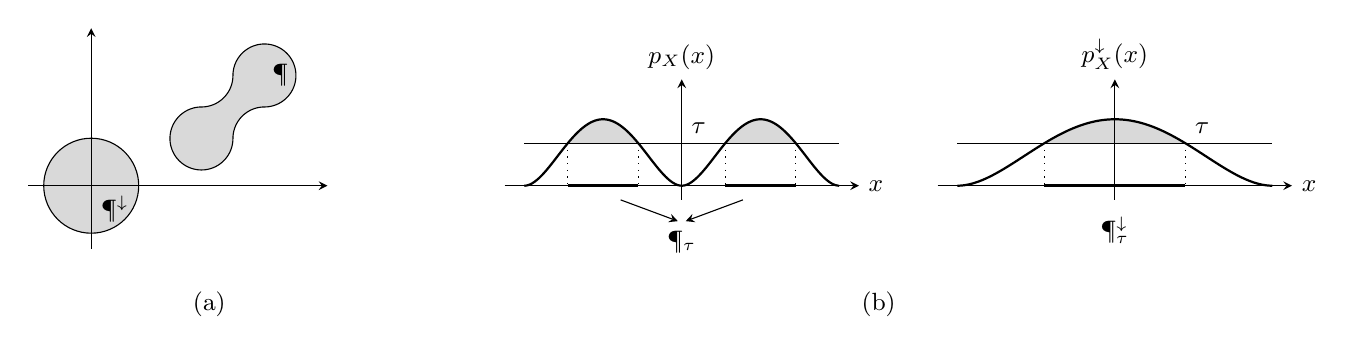
\begin{tikzpicture}
\shorthandoff{>}
%
\begin{scope}[scale=.4]
% Superficia 2*3 pi/4  + 2*2 - 2*pi/4 = 4+pi
\filldraw[draw=black,fill=gray!30]
   plot [domain=0:-270,samples=200] ({cos(\x)+3.5},{sin(\x)+1.5})
-- plot [domain=-90:0,samples=200] ({cos(\x)+3.5},{sin(\x)+3.5})
-- plot [domain=180:-90,samples=200] ({cos(\x)+5.5},{sin(\x)+3.5})
-- plot [domain=90:180,samples=200] ({cos(\x)+5.5},{sin(\x)+1.5})
-- cycle;
\draw (6,3.5) node {\small $\P$};
%
% superficia rearreglada
\filldraw[draw=black,fill=gray!30] (0,0) circle ({sqrt(1+4/pi)});
\draw (.75,-.75) node {\small $\P^\downarrow$};
%
% ejes
\draw[>=stealth,->] (-2,0)--(7.5,0);
\draw[>=stealth,->] (0,-2)--(0,5);
%
\end{scope}
%
%
%----------------------------------------
%
% p_X(x), P_tau...
\begin{scope}[xshift=7.5cm,yscale=1.8]
\pgfmathsetmacro{\t}{.3};
\pgfmathsetmacro{\xt}{sqrt(1-sqrt(32*\t/15))};
\pgfmathsetmacro{\dx}{5.5};% shift para p*(x)
\pgfmathdeclarefunction{studr}{1}{\pgfmathparse{(15/32)*((1-(#1)^2)^2)}}; %Student-r
%
% mezcla de Student-r 15/16 * (1-x^2)^2 (nu = 5) centrados en -1 y 1
% 15/32 (1-(x-a)^2)^2 > t iif (x-a)^2 < 1-sqrt(32*t/15)
% i.e. a-sqrt(1-sqrt(32*t/15)) < x < a+sqrt(1-sqrt(32*t/15))
\fill[domain=-1-\xt:-1+\xt,fill=gray!30] plot(\x,{studr(\x+1)}); % p(x) > tau, x < 0
\fill[domain=1-\xt:1+\xt,fill=gray!30] plot(\x,{studr(\x-1)}); % p(x) > tau, x > 0
\draw[thick,domain=-2:0,samples=100] plot(\x,{studr(\x+1)}); % p(x), x < 0
\draw[thick,domain=0:2,samples=100] plot(\x,{studr(\x-1)}); % p(x), x > 0
\draw (-2,\t)--(2,\t); \draw (0,\t) node[above right]{\small $\tau$}; % y = tau
%
% dominio P_tau
\draw[dotted] ({-1-\xt},{studr(\xt)})--({-1-\xt},0);
\draw[dotted] ({-1+\xt},{studr(\xt)})--({-1+\xt},0);
\draw[very thick] ({-1-\xt},0)--({-1+\xt},0);
\draw[>=stealth,->] ({-1+\xt/2},-.1)--(-.05,-.25);
%
\draw[dotted] ({1-\xt},{studr(\xt)})--({1-\xt},0);
\draw[dotted] ({1+\xt},{studr(\xt)})--({1+\xt},0);
\draw[very thick] ({1-\xt},0)--({1+\xt},0);
\draw[>=stealth,->] ({1-\xt/2},-.1)--(.05,-.25);
%
\draw (0,-.25) node[below]{\small $\P_\tau$};
%
% ejes
\draw[>=stealth,->] (-2.25,0)--(2.25,0) node[right]{\small $x$};
\draw[>=stealth,->] (0,-.1)--(0,.75) node[above]{\small $p_X(x)$};
%
%---------------------------
%
% 15/32 (1-(x-a)^2)^2 > t iif (x-a)^2 < 1-sqrt(32*t/15)
% i.e. a-sqrt(1-sqrt(32*t/15)) < x < a+sqrt(1-sqrt(32*t/15))
% Volumen 2*sqrt(1-sqrt(32*t/15))
% Por simetria, P_t* = [-2*sqrt(1-sqrt(32*t/15)) , 2*sqrt(1-sqrt(32*t/15))]
% da f*(x) = 15/32 (1-x^2/4)^2
\fill[domain=-2*\xt:2*\xt,fill=gray!30] plot({\x+\dx},{studr(.5*\x)}); % p*(x) > tau
\draw[thick,domain=-2:2,samples=200] plot({\x+\dx},{studr(.5*\x)});
\draw ({-2+\dx},\t)--({2+\dx},\t); \draw ({2*\xt+\dx},\t) node[above right]{\small $\tau$}; % y = tau
%
% dominio P_tau*
\draw[dotted] ({-2*\xt+\dx},{studr(\xt)})--({-2*\xt+\dx},0);
\draw[dotted] ({2*\xt+\dx},{studr(\xt)})--({2*\xt+\dx},0);
\draw[very thick] ({-2*\xt+\dx},0)--({2*\xt+\dx},0);
%
\draw (\dx,-.15) node[below]{\small $\P_\tau^\downarrow$};
%
% ejes
\draw[>=stealth,->] ({-2.25+\dx},0)--({2.25+\dx},0) node[right]{\small $x$};
\draw[>=stealth,->] (\dx,-.1)--(\dx,.75) node[above]{\small $p_X^\downarrow(x)$};
\end{scope}
%
\draw (1.5,-1.5) node{\small (a)};
\draw (10,-1.5) node{\small (b)};
\end{tikzpicture} \end{center}
%
\leyenda{(a):  Ilustraci\'on  del rearreglo  sim\'etrico  $\P^\downarrow$ de  un
  conjunto $\P$, siendo  $\P^\downarrow$ la bola centrada en  0 de mismo volumen
  que $\P$, en el caso bi-dimensional $d = 2$.  (b) Construcci\'on del rearreglo
  $p_X^\downarrow$       \modif{en      un      contexto       escalar      (ver
    ejemplo~\ref{Ej:MP:Rearreglo} para $d  = 1, \: \nu = 5, \:  m = 1$)}: dado
  un  $\tau$, se busca  $\P_\tau$ (izquierda)  y se  deduce $\P_\tau^\downarrow$
  (derecha); dado un $x$, se busca el mayor $t$ tal que $x \in \P_t^\downarrow$,
  siendo  entonces  este $t$  m\'aximo  igual  a $p_X^\downarrow(x)$  (derecha);
  adem\'as, por construcci\'on, las superficies en grise son iguales.}
  %
\label{Fig:MP:ensemblerearreglado}
\end{figure}
% =  \B  \left( 0  , r_\P  \right)$ con  $\frac{2
%    \pi^{d/2} r_\P^d}{\Gamma(d/2)} = |\P|$.
\modif{Notar  que, por  construcci\'on, $p_X^\downarrow$  cae el  la  familia de
  densidades  esfericas (ver  secci\'on~\ref{Sec:MP:EjemplosDistribucionesProb})~\cite{Lor54,  FanKot90,
    CamHua81, Eat81}.}

A partir de esta definici\'on del rearreglo, se puede ahora extender la noci\'on
de mayorizaci\'on del caso discreto al caso continuo de la manera siguiente:
%
\begin{definicion}[Mayorizaci\'on en el contexto continuo]
\label{Def:MP:MayorizacionContinua}
%
Una densidad de  probabilidad $p$ se dice mayorizada  por una distribuci\'on $q$
sii:
  %
  \[
  p \prec  q \qquad \mbox{sii}  \qquad \int_{\Bset_d(0,r)} p^\downarrow(x) \,  dx \le
  \int_{\Bset_d(0,r)} q^\downarrow(x) \, dx \quad \forall  \, r > 0, \quad \mbox{ y }
  \quad \int_{\Rset^d} p^\downarrow(x) \, dx = \int_{\Rset^d} q^\downarrow(x) \,
  dx,
  \]
  %
  %donde \ $\B(0,r) = \{ x \in \Rset^d:  \: \|x\| lge r \}$ \ es la bola centrada
  %en \ $0$ \ y de rayo  \ $r$ \ 
  (las \'ultimas integrales son obviamente iguales a 1).
\end{definicion}
%

\modif{Nota:  la  funci\'on   \
%
\[
\L_p(r)  = \int_{\Bset_d(0,r)}  p^{\downarrow}(x) \,  dx
%
\]
%
da el equivalente de  la curba de Lorentz en el contexto  continuo, as\'i que la
relaci\'on de mayorizaci\'on  se interpreta graficamente de la  misma manera que
en el caso  discreto (excepto que, contrariamente al caso  discreto, la curva no
es necesariamente concava).

\begin{ejemplo}\label{Ej:MP:Rearreglo}
  Consideramos la densidad de probabilidad $d$-dimensional \SZ{(mezcla de Student-r;
  ver secci\'on~\ref{Sec:MP:EjemplosDistribucionesProb})}
%
\[
\displaystyle  p_X(x) =  \alpha \left(  \left( 1  - \left\|  x +  m \right\|^2
  \right)^{\frac{\nu-d}{2}} \un_{\Bset_d(-m,1)}(x)  + \left(  1 - \left\|  x -
      m \right\|^2 \right)^{\frac{\nu-d}{2}} \un_{\Bset_d(m,1)}(x)\right)
\]
%
con
%
\[
\nu > d-2, \qquad m \in  \Rset^d \setminus \Bset_d \qquad \mbox{y} \qquad \alpha
=   \frac{\Gamma\left(  \frac{\nu}{2}  +   1  \right)}{2   \,  \pi^{\frac{d}{2}}
  \Gamma\left(   \frac{\nu-d}{2}  +  1   \right)}  \quad   \mbox{coeficiente  de
  normalizaci\'on}
\]
%
Esta         densidad         de         probabilidad        es         dibujada
figura~\ref{Fig:MP:ensemblerearreglado}-((b) izquierda) para $d = 1, \: \nu = 5,
m = 1$ y  figura~\ref{Fig:MP:RearregloMayorizacionEjemplo}-(a) para $d = 2, \:
\nu  = 6,  \: m  = \frac{1}{\sqrt{d}}  \un$.  El  dominio de  definici\'on, el
m\'aximo,       y       la       matriz       de       covarianza       \SZ{(ver
  secci\'on~\ref{Sec:MP:EjemplosDistribucionesProb})} son dados por
%
\[
\X = \Bset_d(-m,1) \: \cup  \: \Bset_d(m,1), \qquad \max_\X p_X(x) = \alpha,
\qquad \Sigma_X = \frac{1}{\nu+2} I + m m^t
\]

Ahora, para \ $\tau  > \alpha, \: \P_\tau = \emptyset$ \  y para cualquier $\tau
\in [0 \; \alpha]$  buscando los $x$ tal que $p_X(x) >  \tau$ (notando que las
bolas en $\X$ son disjuntas) conduce a
%
\[
\P_\tau = \Bset_d(-m , \beta_\tau) \: \cup \: \Bset_d(m , \beta_\tau) \qquad
\mbox{con} \qquad  \beta_\tau = \sqrt{  1 - \left( \frac{2  \, \pi^{\frac{d}{2}}
      \Gamma\left(    \frac{\nu-d}{2}   +1    \right)    \,   \tau}{\Gamma\left(
        \frac{\nu}{2} +1 \right)} \right)^{\frac{2}{\nu-d}}}
\]
%
Notando  que las esferas  de \  $\P_\tau$ \  son disjuntas,  queda claro  que el
volumen de  \ $\P_\tau$ \ es  dado por \ $\left|  \P_\tau \right| =  2 \, \left|
  \Bset_d\left(  0 ,  \beta_\tau  \right)  \right| =  \left|  \Bset_d\left( 0  ,
    2^{\frac{1}{d}}   \beta_\tau  \right)  \right|$,   que  conduce   al  dominio
  rearreglado,
%
\[
\P^{\downarrow}_\tau  =  \Bset_d\left( 0  ,  2^{\frac{1}{d}}  \beta_\tau \right)
\]
%
Ahora, se muestra sencillamente que $x \in \P^{\downarrow}_u$ es equivalente a
%
\[
\displaystyle  u   <  \frac{\Gamma\left(  \frac{\nu}{2}  +   1  \right)}{2  \,
  \pi^{\frac{d}{2}}  \Gamma\left( \frac{\nu-d}{2}  + 1  \right)} \,  \left(  1 -
  \frac{\|x\|^2}{4^{\frac1d}}  \right)^{\frac{\nu-d}{2}}  \un_{\Bset_d\left(0  ,
    2^{\frac1d} \right)}(x)
\]
%
De la definici\'on~\ref{Def:MP:RearregloDensidad} obtenemos al final
 %
 \[
 p^{\downarrow}_X(x)  =  \frac{\Gamma\left(  \frac{\nu}{2}  +  1  \right)}{2  \,
   \pi^{\frac{d}{2}}  \Gamma\left( \frac{\nu-d}{2} +  1 \right)}  \, \left(  1 -
   \frac{\|x\|^2}{4^{\frac1d}}  \right)^{\frac{\nu-d}{2}}  \un_{\Bset_d\left(0 ,
     2^{\frac1d} \right)}(x)
 \]
%
 dibujada figura~\ref{Fig:MP:ensemblerearreglado}-((b) derecha)  para $d = 1, \:
 \nu = 5$ y figura~\ref{Fig:MP:RearregloMayorizacionEjemplo} para $d = 2, \: \nu
 = 6$.
%
Finalmente, la curva de Lorentz es dada por
%
\begin{eqnarray*}
\L_{p_X}(r) & = & \frac{\Gamma\left( \frac{\nu}{2} + 1 \right)}{2 \,
\pi^{\frac{d}{2}} \Gamma\left( \frac{\nu-d}{2} + 1 \right)} \int_{\Bset_d(0,r)}
\left( 1 - \frac{\|x\|^2}{4^{\frac1d}} \right)^{\frac{\nu-d}{2}}
\un_{\Bset_d\left(0 , 2^{\frac1d} \right)}(x) \, dx\\
%
& = & \frac{\Gamma\left( \frac{\nu}{2} + 1 \right)}{2 \, \pi^{\frac{d}{2}}
\Gamma\left( \frac{\nu-d}{2} + 1 \right)} \frac{2 \,
\pi^{\frac{d}{2}}}{\Gamma\left( \frac{d}{2} \right)} \int_0^r \rho^{d-1} \left( 1 -
\frac{\rho^2}{4^{\frac1d}} \right)^{\frac{\nu-d}{2}} \un_{\left[ 0 \; 2^{\frac1d}
\right]}(\rho) \, d\rho
\end{eqnarray*}
%
pasando  en coordenadas  hiperesferica (ver~\cite{Lor54,  FanKot90,  CamHua81} y
secci\'on~\ref{Sec:MP:EjemplosDistribucionesProb}). Por el cambio de variable $u
= \frac{\rho^2}{4^{\frac1d}}$ obtenemos
%
\[
\L_{p_X}(r)      =      \frac{\displaystyle     \int_0^{\frac{r^2}{4^{\frac1d}}}
  u^{\frac{d}{2}-1} (1-u)^{\frac{\nu-d}{2}}  \, du}{B\left( \frac{d}{2}  \, , \,
    \frac{\nu-d}{2} + 1 \right)}
\]
%
conocida  como funci\'on  beta incompleta~\cite[Ec.~8.392]{GraRyz15},  tomada en
$\frac{r^2}{4^{\frac1d}}$.                                                     La
figura~\ref{Fig:MP:RearregloMayorizacionEjemplo}-(c)  dibuja  $\L_{p_X}(r)$ para
$d  = 2,  \: \nu  =  6$, la  de la  ley  gausiana esferica  $g_X$ de  covarianza
$\frac{\Tr \Sigma_X}{d} I$ y la de la ley Student-t esferica $s_X$ de covarianza
$\frac{\Tr  \Sigma_X}{d} I$  y con  \ $\nu'  = 2.25$  \ grado  de  libertad (ver
secci\'on~\ref{Sec:MP:EjemplosDistribucionesProb}). Eso  ilustra graficamente la
relaci\'on de  mayorizaci\'on \ $g_X \prec p_X$  \ y que ambas  \ $s_X \not\prec
p_X$ \ y \ $p_X \not\prec s_X$.
% $p(x) = \frac{}{}$$ y la ley arcsin $q_X(x) = $

\begin{figure}[h!]
\begin{center} \begin{tikzpicture}%[scale=.8]
\shorthandoff{>}
%
\tikzset{declare function={
xplus(\x) = max(\x,0);
%ifthenelse(\x > 0 , \x , NaN);
}}
%
% Approximation de la cdf gaussienne
\tikzset{declare function={
normcdf(\x)=1/(1 + exp(-0.07056*(\x)^3 - 1.5976*(\x)));
}}
%
% gamma incompleta para k entero
\tikzmath{function gammainc(\x,\k) {
    if \k == 1 then {return (1-exp(-\x));}
    else {return gammainc(\x,\k-1)*(\k-1)-((\x)^(\k-1))*exp(-\x);};
};};
%
%
% beta incompleta (k,l) int_0^r u^(k-1) (1-u)^() para l entero, k > 0
\tikzmath{function betainc(\x,\k,\l) {
    if \x <= 0 then {return 0;}
    else {if \x > 1 then {return betainc(1,\k,\l);}
          else {if \l == 1 then {return ((\x)^(\k))/\k;}
                else {return ((\l-1)/\k)*betainc(\x,\k+1,\l-1)+(((\x)^(\k))*((1-\x)^(\l-1))/\k);};
               };
         };
};};
%
\pgfmathsetmacro{\d}{2};% dimension
\pgfmathsetmacro{\nu}{6};% degres de liberte
\pgfmathsetmacro{\mux}{1/sqrt(2)};% mu_1
\pgfmathsetmacro{\muy}{1/sqrt(2)};% mu_2
\pgfmathsetmacro{\a}{factorial(\nu/2)/(2*(pi^(\d/2))*factorial((\nu-\d)/2))};

\tdplotsetmaincoords{45}{65}
\begin{scope}[tdplot_main_coords,scale=.65]
%
% densidad d=2, nu = 4, mu = [1 1]/sqrt(2)
% Mezcla de Student-r
\begin{axis}[
    colormap = {whiteblack}{color(0cm)  = (white);color(1cm) = (black)},
    width=.5\textwidth,
    view={45}{65},
    enlargelimits=false,
    %grid=major,
    domain=-2.5:2.5,
    y domain=-2.5:2.5,
    zmax={.85*\a},
    color=black,
    samples=70,
    xlabel=$x_1$,
    ylabel=$x_2$,
    zlabel=$p_X$,
]
%
% Mezcla de Student
\addplot3 [surf] {
\a*((xplus(1-(x+\mux)^2-(y+\muy)^2))^((\nu-\d)/2)+(xplus(1-(x-\mux)^2-(y-\muy)^2))^((\nu-\d)/2))};
%%
\end{axis}
\end{scope}
%
%
% densidad rearreglada
\begin{scope}[tdplot_main_coords,xshift=5.5cm,scale=.65]
%
\begin{axis}[
    colormap = {whiteblack}{color(0cm)  = (white);color(1cm) = (black)},
    width=.5\textwidth,
    view={45}{65},
    enlargelimits=false,
    %grid=major,
    domain=-2:2,
    y domain=-2:2,
    zmax={.8*\a},
    color=black,
    samples=70,
    xlabel=$x_1$,
    ylabel=$x_2$,
    zlabel=$p^{\downarrow}_X$,
]
%
% Mezcla rearreglada
\addplot3 [surf,opacity=.8] {\a*((xplus(1-(x^2+y^2)/(4^(1/\d))))^((\nu-\d)/2))};
%
\end{axis}
\end{scope}
%
% curva de Lorentz
\begin{scope}[xshift=11.25cm,yshift=.5cm,scale=.65]
\pgfmathsetmacro{\sx}{1.5};% x-scaling
\pgfmathsetmacro{\sy}{2.75};% y-scaling 
\pgfmathsetmacro{\mx}{3.25};% maximo en x
\pgfmathsetmacro{\B}{betainc(1,\d/2,(\nu-\d)/2+1)};% B(d/2,(nu-d)/2+1)
\pgfmathsetmacro{\ss}{(1/(\nu+2))+(((\mux)^2)+((\muy)^2))/\d};
\pgfmathsetmacro{\nut}{2.25};% nu Student-t
\pgfmathsetmacro{\Bt}{betainc(1,\nut/2,\d/2)};% B(d/2,nust/2)
\pgfmathsetmacro{\st}{(\nut-2)*((1/(\nu+2))+(((\mux)^2)+((\muy)^2))/\d)};

\draw[>=stealth,->] (-.25,0)--({\sx*\mx+.5},0) node[right]{\small $r$};
\draw[>=stealth,->] (0,-.15)--(0,{\sy+.5}) node[above]{\small $\L_p(r)$};
%

% Lorentz de la mezcla
\draw[thick,domain=0:\mx,samples=50,smooth] plot({\x*\sx},{\sy*betainc(((\x)^2)/(4^(1/\d)),\d/2,(\nu-\d)/2+1)/\B});
%
% Lorentz de la gausiana
\draw[thick,dashed,domain=0:\mx,samples=50,smooth] plot({\x*\sx},{\sy*gammainc(((\x)^2)/2/\ss,\d/2)/factorial(\d/2-1)});
%
% Lorentz de la student-t nu' = 3;
\draw[thick,dotted,domain=0:\mx,samples=50,smooth] plot({\x*\sx},{\sy*betainc(((\x)^2)/(\st+(\x)^2),\nut/2,\d/2)/\Bt});
%
\foreach \m in {0,...,\mx} {
\draw ({\m*\sx},0)--({\m*\sx},-.1) node[below,scale=.7]{$\m$};
}
%
\draw (0,\sy)--(-.1,\sy) node[left,scale=.7]{$1$};
\end{scope}
%
\node at (2.05,-.75){(a)};
\node at (7.55,-.75){(b)};
\node at (13,-.75){(c)};
\end{tikzpicture} \end{center}
%
\leyenda{(a) Densidad de probabilidad $p_X$ del ejemplo~\ref{Ej:MP:Rearreglo} en
  el contexto bi-dimensional $d = 2$ y  para $\nu = 6, \: m = \frac{1}{\sqrt{d}}
  \un$. (b) Densidad rearreglada $p^{\downarrow}_X$. (c) Equivalente continua de
  la curva de Lorentz para la densidad $p_X$ (linea llena), la densidad gausiana
  esferica \ $g_X$  \ con covarianza de  misma traza que la de  $p_X$ (linea con
  guiones) y  la densidad Student-t  \ con covarianza  de misma traza que  la de
  $p_X$ \ y \  $\nu' = 2.25$ \ grado de libertad  (linea punteada): \ $g_X \prec
  p_X$ \ pero \ $s_X \not\prec p_X$ \ y \ $p_X \not\prec s_X$.}
\label{Fig:MP:RearregloMayorizacionEjemplo}
\end{figure}
\end{ejemplo}
}